%  LaTeX support: latex@mdpi.com 
%  For support, please attach all files needed for compiling as well as the log file, and specify your operating system, LaTeX version, and LaTeX editor.

%=================================================================
\documentclass[journal,article,submit,pdftex,moreauthors]{Definitions/mdpi} 

%--------------------
% Class Options:
%--------------------
%----------
% journal
%----------
% Choose between the following MDPI journals:
% acoustics, actuators, addictions, admsci, adolescents, aerobiology, aerospace, agriculture, agriengineering, agrochemicals, agronomy, ai, air, algorithms, allergies, alloys, analytica, analytics, anatomia, animals, antibiotics, antibodies, antioxidants, applbiosci, appliedchem, appliedmath, applmech, applmicrobiol, applnano, applsci, aquacj, architecture, arm, arthropoda, arts, asc, asi, astronomy, atmosphere, atoms, audiolres, automation, axioms, bacteria, batteries, bdcc, behavsci, beverages, biochem, bioengineering, biologics, biology, biomass, biomechanics, biomed, biomedicines, biomedinformatics, biomimetics, biomolecules, biophysica, biosensors, biotech, birds, bloods, blsf, brainsci, breath, buildings, businesses, cancers, carbon, cardiogenetics, catalysts, cells, ceramics, challenges, chemengineering, chemistry, chemosensors, chemproc, children, chips, cimb, civileng, cleantechnol, climate, clinpract, clockssleep, cmd, coasts, coatings, colloids, colorants, commodities, compounds, computation, computers, condensedmatter, conservation, constrmater, cosmetics, covid, crops, cryptography, crystals, csmf, ctn, curroncol, cyber, dairy, data, ddc, dentistry, dermato, dermatopathology, designs, devices, diabetology, diagnostics, dietetics, digital, disabilities, diseases, diversity, dna, drones, dynamics, earth, ebj, ecologies, econometrics, economies, education, ejihpe, electricity, electrochem, electronicmat, electronics, encyclopedia, endocrines, energies, eng, engproc, entomology, entropy, environments, environsciproc, epidemiologia, epigenomes, est, fermentation, fibers, fintech, fire, fishes, fluids, foods, forecasting, forensicsci, forests, foundations, fractalfract, fuels, future, futureinternet, futurepharmacol, futurephys, futuretransp, galaxies, games, gases, gastroent, gastrointestdisord, gels, genealogy, genes, geographies, geohazards, geomatics, geosciences, geotechnics, geriatrics, grasses, gucdd, hazardousmatters, healthcare, hearts, hemato, hematolrep, heritage, higheredu, highthroughput, histories, horticulturae, hospitals, humanities, humans, hydrobiology, hydrogen, hydrology, hygiene, idr, ijerph, ijfs, ijgi, ijms, ijns, ijpb, ijtm, ijtpp, ime, immuno, informatics, information, infrastructures, inorganics, insects, instruments, inventions, iot, j, jal, jcdd, jcm, jcp, jcs, jcto, jdb, jeta, jfb, jfmk, jimaging, jintelligence, jlpea, jmmp, jmp, jmse, jne, jnt, jof, joitmc, jor, journalmedia, jox, jpm, jrfm, jsan, jtaer, jvd, jzbg, kidneydial, kinasesphosphatases, knowledge, land, languages, laws, life, liquids, literature, livers, logics, logistics, lubricants, lymphatics, machines, macromol, magnetism, magnetochemistry, make, marinedrugs, materials, materproc, mathematics, mca, measurements, medicina, medicines, medsci, membranes, merits, metabolites, metals, meteorology, methane, metrology, micro, microarrays, microbiolres, micromachines, microorganisms, microplastics, minerals, mining, modelling, molbank, molecules, mps, msf, mti, muscles, nanoenergyadv, nanomanufacturing,\gdef\@continuouspages{yes}} nanomaterials, ncrna, ndt, network, neuroglia, neurolint, neurosci, nitrogen, notspecified, %%nri, nursrep, nutraceuticals, nutrients, obesities, oceans, ohbm, onco, %oncopathology, optics, oral, organics, organoids, osteology, oxygen, parasites, parasitologia, particles, pathogens, pathophysiology, pediatrrep, pharmaceuticals, pharmaceutics, pharmacoepidemiology,\gdef\@ISSN{2813-0618}\gdef\@continuous pharmacy, philosophies, photochem, photonics, phycology, physchem, physics, physiologia, plants, plasma, platforms, pollutants, polymers, polysaccharides, poultry, powders, preprints, proceedings, processes, prosthesis, proteomes, psf, psych, psychiatryint, psychoactives, publications, quantumrep, quaternary, qubs, radiation, reactions, receptors, recycling, regeneration, religions, remotesensing, reports, reprodmed, resources, rheumato, risks, robotics, ruminants, safety, sci, scipharm, sclerosis, seeds, sensors, separations, sexes, signals, sinusitis, skins, smartcities, sna, societies, socsci, software, soilsystems, solar, solids, spectroscj, sports, standards, stats, std, stresses, surfaces, surgeries, suschem, sustainability, symmetry, synbio, systems, targets, taxonomy, technologies, telecom, test, textiles, thalassrep, thermo, tomography, tourismhosp, toxics, toxins, transplantology, transportation, traumacare, traumas, tropicalmed, universe, urbansci, uro, vaccines, vehicles, venereology, vetsci, vibration, virtualworlds, viruses, vision, waste, water, wem, wevj, wind, women, world, youth, zoonoticdis 
% For posting an early version of this manuscript as a preprint, you may use "preprints" as the journal. Changing "submit" to "accept" before posting will remove line numbers.

%---------
% article
%---------
% The default type of manuscript is "article", but can be replaced by: 
% abstract, addendum, article, book, bookreview, briefreport, casereport, comment, commentary, communication, conferenceproceedings, correction, conferencereport, entry, expressionofconcern, extendedabstract, datadescriptor, editorial, essay, erratum, hypothesis, interestingimage, obituary, opinion, projectreport, reply, retraction, review, perspective, protocol, shortnote, studyprotocol, systematicreview, supfile, technicalnote, viewpoint, guidelines, registeredreport, tutorial
% supfile = supplementary materials

%----------
% submit
%----------
% The class option "submit" will be changed to "accept" by the Editorial Office when the paper is accepted. This will only make changes to the frontpage (e.g., the logo of the journal will get visible), the headings, and the copyright information. Also, line numbering will be removed. Journal info and pagination for accepted papers will also be assigned by the Editorial Office.

%------------------
% moreauthors
%------------------
% If there is only one author the class option oneauthor should be used. Otherwise use the class option moreauthors.

%---------
% pdftex
%---------
% The option pdftex is for use with pdfLaTeX. Remove "pdftex" for (1) compiling with LaTeX & dvi2pdf (if eps figures are used) or for (2) compiling with XeLaTeX.

%=================================================================
% MDPI internal commands - do not modify
\firstpage{1} 
\makeatletter 
\setcounter{page}{\@firstpage} 
\makeatother
\pubvolume{1}
\issuenum{1}
\articlenumber{0}
\pubyear{2024}
\copyrightyear{2024}
%\externaleditor{Academic Editor: Firstname Lastname}
% \datereceived{ } 
% \daterevised{ } % Comment out if no revised date
% \dateaccepted{ } 
% \datepublished{ } 
%\datecorrected{} % For corrected papers: "Corrected: XXX" date in the original paper.
%\dateretracted{} % For corrected papers: "Retracted: XXX" date in the original paper.
% \hreflink{https://doi.org/} % If needed use \linebreak
%\doinum{}
%\pdfoutput=1 % Uncommented for upload to arXiv.org
%\CorrStatement{yes}  % For updates


%=================================================================
% Add packages and commands here. The following packages are loaded in our class file: fontenc, inputenc, calc, indentfirst, fancyhdr, graphicx, epstopdf, lastpage, ifthen, float, amsmath, amssymb, lineno, setspace, enumitem, mathpazo, booktabs, titlesec, etoolbox, tabto, xcolor, colortbl, soul, multirow, microtype, tikz, totcount, changepage, attrib, upgreek, array, tabularx, pbox, ragged2e, tocloft, marginnote, marginfix, enotez, amsthm, natbib, hyperref, cleveref, scrextend, url, geometry, newfloat, caption, draftwatermark, seqsplit
% cleveref: load \crefname definitions after \begin{document}
\preto{\abstractkeywords}{\nolinenumbers}

%=================================================================
% Please use the following mathematics environments: Theorem, Lemma, Corollary, Proposition, Characterization, Property, Problem, Example, ExamplesandDefinitions, Hypothesis, Remark, Definition, Notation, Assumption
%% For proofs, please use the proof environment (the amsthm package is loaded by the MDPI class).

%=================================================================
% Full title of the paper (Capitalized)
\Title{Strip It To The Bone: In-Depth Study of Soft Tissue Thickness for Forensic Analysis}

%\Title{Strip It To The Bone: In-Depth Analysis of Soft Tissue Thickness for Forensic Facial Reconstruction}

% MDPI internal command: Title for citation in the left column
\TitleCitation{Strip It To The Bones: In-Depth Study of Soft Tissue Thickness for Forensic Analysis}

% Author Orchid ID: enter ID or remove command
\newcommand{\orcidauthorA}{0000-0000-0000-000X} % Add \orcidA{} behind the author's name
%\newcommand{\orcidauthorB}{0000-0000-0000-000X} % Add \orcidB{} behind the author's name

% Authors, for the paper (add full first names)
\Author{GROUP 15. Federica Amato $^{1,\dagger}$, Matteo Di Iorio $^{1,\dagger}$, Antonio Ferrigno $^{1,\dagger}$, Giulio Figliolino $^{1,\dagger}$ and Fatjona Gjikopulli $^{1,\dagger}$}

%\longauthorlist{yes}

% MDPI internal command: Authors, for metadata in PDF
\AuthorNames{Federica Amato, Matteo Di Iorio, Antonio Ferrigno, Giulio Figliolino and Fatjona Gjikopulli}

% MDPI internal command: Authors, for citation in the left column
\AuthorCitation{Amato, F.; Di Iorio, M.; Ferrigno, A.; Figliolino, G.; Gjikopulli, F.}
% If this is a Chicago style journal: Lastname, Firstname, Firstname Lastname, and Firstname Lastname.

% Affiliations / Addresses (Add [1] after \address if there is only one affiliation.)
\address{[1]
\quad Polytechnic University of Turin, Corso Duca degli Abruzzi 24, 10129 Turin, Italy; s310275@studenti.polito.it (F.A.); s316606@studenti.polito.it (M.D.I.); s316467@studenti.polito.it (A.F.); s317510@studenti.polito.it (G.F.); s317496@studenti.polito.it (F.G.)}

% Contact information of the corresponding author
% \corres{Correspondence: e-mail@e-mail.com; Tel.: (optional; include country code; if there are multiple corresponding authors, add author initials) +xx-xxxx-xxx-xxxx (F.L.)}

% Current address and/or shared authorship
% \firstnote{Current address: Affiliation.}  % Current address should not be the same as any items in the Affiliation section.
\firstnote{These authors contributed equally to this work.}
% The commands \thirdnote{} till \eighthnote{} are available for further notes

%\simplesumm{} % Simple summary

%\conference{} % An extended version of a conference paper

% Abstract (Do not insert blank lines, i.e. \\) 
\abstract{Forensic facial reconstruction (FFR) is crucial for identifying human remains in medico-legal context, but the variability in facial soft tissue thickness (FSTT) due to demographic factors like age, sex, and body mass index (BMI) persists as an open problem. This study employs high-resolution DICOM data to accurately measure FSTT at craniofacial landmarks, examining a sample of 57 patients (36 males, 21 females). The segmentation and mesh filtering process facilitated precise measurements. Statistical analysis using Pearson correlation coefficient and ANCOVA, along with Machine Learning models like Random Forest (RF) and Decision Tree (DT), confirmed that BMI significantly influences FSTT, with higher BMI correlating with increased tissue thickness, particularly in the mid-philtrum regions. Age and sex showed a lesser but still significant impact. These results confirm the importance of considering individual demographic characteristics to improve the accuracy of FFRs and surgical planning. This rigorous methodological approach ensures reliable and applicable results in both forensic and medical contexts, proposing a significant improvement in facial reconstruction techniques based on detailed FSTT analysis.}

% Keywords
\keyword{soft tissue thickness; DICOM data; 3D landmarks;
statistical analysis; forensic facial reconstruction; Random Forest Algorithm; Decision Tree; ANCOVA; Linear Regression; Pearson correlation coefficient}

% The fields PACS, MSC, and JEL may be left empty or commented out if not applicable
%\PACS{J0101}
%\MSC{}
%\JEL{}

%%%%%%%%%%%%%%%%%%%%%%%%%%%%%%%%%%%%%%%%%%
% Only for the journal Diversity
%\LSID{\url{http://}}

%%%%%%%%%%%%%%%%%%%%%%%%%%%%%%%%%%%%%%%%%%
% Only for the journal Applied Sciences
%\featuredapplication{Authors are encouraged to provide a concise description of the specific application or a potential application of the work. This section is not mandatory.}
%%%%%%%%%%%%%%%%%%%%%%%%%%%%%%%%%%%%%%%%%%

%%%%%%%%%%%%%%%%%%%%%%%%%%%%%%%%%%%%%%%%%%
% Only for the journal Data
%\dataset{DOI number or link to the deposited data set if the data set is published separately. If the data set shall be published as a supplement to this paper, this field will be filled by the journal editors. In this case, please submit the data set as a supplement.}
%\datasetlicense{License under which the data set is made available (CC0, CC-BY, CC-BY-SA, CC-BY-NC, etc.)}

%%%%%%%%%%%%%%%%%%%%%%%%%%%%%%%%%%%%%%%%%%
% Only for the journal Toxins
%\keycontribution{The breakthroughs or highlights of the manuscript. Authors can write one or two sentences to describe the most important part of the paper.}

%%%%%%%%%%%%%%%%%%%%%%%%%%%%%%%%%%%%%%%%%%
% Only for the journal Encyclopedia
%\encyclopediadef{For entry manuscripts only: please provide a brief overview of the entry title instead of an abstract.}

%%%%%%%%%%%%%%%%%%%%%%%%%%%%%%%%%%%%%%%%%%
% Only for the journal Advances in Respiratory Medicine
%\addhighlights{yes}
%\renewcommand{\addhighlights}{%

%\noindent This is an obligatory section in “Advances in Respiratory Medicine”, whose goal is to increase the discoverability and readability of the article via search engines and other scholars. Highlights should not be a copy of the abstract, but a simple text allowing the reader to quickly and simplified find out what the article is about and what can be cited from it. Each of these parts should be devoted up to 2~bullet points.\vspace{3pt}\\
%\textbf{What are the main findings?}
% \begin{itemize}[labelsep=2.5mm,topsep=-3pt]
% \item First bullet.
% \item Second bullet.
% \end{itemize}\vspace{3pt}
%\textbf{What is the implication of the main finding?}
% \begin{itemize}[labelsep=2.5mm,topsep=-3pt]
% \item First bullet.
% \item Second bullet.
% \end{itemize}
%}

%%%%%%%%%%%%%%%%%%%%%%%%%%%%%%%%%%%%%%%%%%
\begin{document}

%%%%%%%%%%%%%%%%%%%%%%%%%%%%%%%%%%%%%%%%%%
\section{Introduction}
The identification of human remains has been a significant challenge for the medico-legal system. A thorough examination of recovered unidentified skeletal remains provides answers to fundamental questions regarding characteristics such as sex, age, and ethnicity, and helps to address trauma \cite{ref1}. When corpses lack distinctive features and their identities cannot be confirmed through conventional methods, such as DNA analysis, fingerprint analysis, or dental records [due to advanced postmortem decomposition process or insufficient information], facial reconstruction is one of the last options to recreate their antemortem appearance \citep{ref2,ref3,ref4,ref5}.

Forensic facial reconstruction (FFR) plays a crucial role in investigating victims \cite{ref4}. 
%[of genocide and mass disasters, including wars, natural or intentional accidents] \cite{ref4}. 
[The technique involves] assembling an approximate soft tissue topography over the unknown skull to reconstruct [its characteristics as closely as possible to the] individual's appearance at the time of death. Once the reconstruction is complete, a public campaign is launched to elicit responses about the possible identity of the remains. This is followed by a formal identification process \cite{ref3}.

% [Although the terms "facial reconstruction" and "facial approximation" are often used interchangeably, authors nowadays prefer "facial approximation" since it is impossible to precisely reproduce an individual's antemortem appearance.]
The techniques employed to reproduce the face are method specific, which makes the overall process prone to errors, 
%[. Consequently, the practitioner can only approximate the natural appearance at best. As a result, ] 
therefore FFR remains an inherently subjective and contentious process, despite incorporating complex sciences such as forensics, anthropology, osteology, and anatomy \cite{ref6}.

[The anthropometric or American Approach, also known as the tissue depth method, was devised in 1946 by anthropologist Wilton Marrion Krogman and later refined in the 1970s by forensic artist Betty Pat Gatliff and physical anthropologist Clyde Snow. This method was manual and involved directly modelling and sculpting by applying clay or Plasticine over the skull or a model of the skull.] Similarly, the Manchester or British method, developed by Neave in 1977 [and later revised by Wilkinson], combines soft tissue thickness with basic anatomy to reproduce faces \citep{ref7,ref8,ref9,ref10}.

More recently, computerized face sculptures can be generated using specialized modelling software (digital method) \cite{ref11}.
%, [with various user interfaces designed to mimic manual modelling procedures.] 
% In a 3D context, tablets and haptic devices may be used to add soft tissues to a model of the skull \cite{ref11}.

However, regardless of the method used, it is crucial to establish parameters and guidance such as facial soft tissue thickness (FSTT), as variations in FSTT can significantly influence the facial contours of an individual. The points used to estimate the FSTT are known as craniometric landmarks, or facial landmarks. These landmarks are key points of the face with a certain biometric and geometric significance. They may be either skeletal or soft tissue-based, depending on their location—either on bone or directly on the skin. When located on bone, they are referred to as craniometric landmarks of hard tissue, while those on the skin are termed craniometric landmarks of soft tissue \citep{ref4,ref7,ref12}. Establishing values for FSTT, as well as understanding the relationship between soft and hard tissue, can be achieved through radiological techniques such as X-ray, computed tomography (CT), nuclear magnetic resonance (NMR), and ultrasound. These methods can be conducted in vivo or on cadaveric material, with the latter involving direct measurement via needle puncture \citep{ref13,ref14,ref15,ref16,ref17,ref18}.

Piombino et al. \cite{ref19} carried out a comprehensive analysis of FSTT, focusing on the effects of age, sex, and body mass index (BMI). Measurements were conducted on cone beam computed tomography (CBCT). Their results revealed that BMI plays a significant role at various craniometric points, with higher BMI generally leading to increased FSTT, especially in areas like the mid-philtrum [and prosthion]. In contrast, age and sex have a more marginal yet significant/useful impact.

During the same period, the study undertaken by Park et al. \cite{ref2} involved malocclusion 102 patients in their 20s. They were divided into three skeletal classes based on CBCT data and the ANB angle, which indicates the position of the maxilla in relation to the mandible. FSTT was compered between genders and across skeletal classes. Key findings indicated that males generally have thicker FSTT than females across all skeletal types. This aligns with previous research suggesting that men have larger bones and muscles, and testosterone promotes collagen synthesis, making men’s skin thicker.

Other studies, even older ones, focused on the same theme, yielding results that have been pivotal for subsequent research. Ellie Simpson and Maciej Henneberg \cite{ref20} investigated the relationship between facial soft tissue depths and cranial morphology. Measurements were taken on adult, white Australian cadavers. The findings revealed significant correlations between FSTT and the size of the underlying cranial structure. Males exhibited thicker soft tissues and larger craniometric dimensions compared to females (in accordance with the study conducted in South Korea), though there was considerable overlap of ranges. Additionally, the study examined the impact of tissue embalming, noting significant initial increases in facial soft tissue depths due to this process. These findings hold implications for forensic identification and the estimation of facial features in extinct populations.

Another research [aimed to develop a specific database for the Romanian adult population] by investigating the statistical distribution and correlations of craniometric landmarks, conducted by Diac et al \cite{ref21}. The authors categorized these landmarks by sex and weight to assist in estimating missing landmark values for unidentified bodies. Measurements were taken on twelve landmarks from 100 cadavers within 24 hours of death. Results showed significant sex-related differences in one landmark and significant variations across different weight categories in seven landmarks. The study also found evidence in average FSTT compared to similar studies involving Caucasian groups from diverse geographic origins.

Indeed, in recent years, studies have shown that FSTT data can vary notably also among different population groups \citep{ref13,ref22,ref23,ref24,ref25}, yet consensus on this topic remains elusive. Thus, several countries 
%[(France, Brazil, Portugal, etc.)] 
have conducted and/or are conducting extensive research to establish FSTT values, specific to each population \citep{ref13,ref14,ref15,ref16,ref17,ref18}. Moritsugui et al. \cite{ref26} sought to assess the impact of regional differences within Brazil on FSTT, crucial for FFR. Researchers employed a specific CBCT protocol to standardize measurements across a sample of 101 subjects. High compatibility was observed when comparing the avarages of FSTT among samples of two different geographic regions, Midwest and Southeast regions. Regarding age groups, notable differences on the medium and inferior face were observed in females. Therefore, distinct datasets for the Southeast and Midwest regions of Brazil are unnecessary.

Despite advancements in imaging techniques and the availability of high-resolution data, there remains a scarcity of studies that have conducted comprehensive statistical analyses on the correlation between variables such as age, sex, and BMI with FSTT, particularly using CBCT measurements. Recognizing the variability in methodologies, including original measurement protocols, imaging exam sources and types, and regional chart relations, alongside the uncertain success of the FFR, poses challenges for comparing and validating results across studies. Therefore, this study advocates for further investigation into the influence of these variables on FSTT to improve the management of FFR procedures. The primary objectives include the following:

% This project aims to address these challenges by utilizing DICOM data to accurately measure FSTT at defined facial landmarks and perform statistical analyses to assess variations based on gender, age and BMI. The results will be benchmarked against established data to ensure reliability and validity, thereby enhancing the credibility and applicability of the findings in real-world scenarios. The primary objectives of this study include:

\begin{enumerate}
    \item Utilizing DICOM data to accurately measure FSTT at defined facial landmarks.
    
    \item Contextualizing these measurements within specific forensic applications, ensuring relevance and practical utility.
    
    \item Performing statistical analyses to assess variations in FSTT based on gender, age, and BMI.
    
    \item Ensuring that FSTT measurement accuracy aligns with current literature standards, facilitating reliable comparisons and validations of results.
\end{enumerate}

The remaining sections of this paper are organized as follows. Section \ref{sec:matmet} elaborates on the use of high-resolution DICOM data for accurate and reproducible measurements, detailing the statistical methods used to examine variations in FSTT. Sections \ref{sec:res} and \ref{sec:disc} present comprehensive results, discussions, and comparisons with recent studies. The final section summarizes the study's key findings, discusses its limitations, and proposes potential avenues for future research or applications.
%%%%%%%%%%%%%%%%%%%%%%%%%%%%%%%%%%%%%%%%%%
\section{Materials and Methods}
\label{sec:matmet}
In this section, the main steps that characterized the analysis will be presented, with references to the methods and strategies adopted.

\subsection{Data collection}

The primary dataset used for this research was sourced from the publicly available collection on Academic Torrents \cite{ref27}. This extracted dataset is a subset of DICOM formats representing CT scans, originally compiled for a study on head and neck cancer. Specifically, the dataset includes FDG-PET/CT and radiotherapy planning CT imaging data for 298 patients from four institutions in Quebec, with histologically proven head-and-neck cancer. These patients had pre-treatment FDG-PET/CT scans between April 2006 and November 2014.\\
%• URL: Head-Neck-CT \\
%• License: Creative Commons Attribution 3.0 Unported License \\
Due to limited time and some CT images being unsuitable for analysis, 43 patients from the initial database were analyzed, of which 29 were men and 14 were women. \\
Additionally, NRRD data from 14 patients (7 males and 7 females) provided by Professor Olivetti and Professor Marcolin were chosen. These patients were evenly distributed across three hospitals.

\begin{figure}[H]
\centering
\begin{minipage}{0.8\textwidth}
\centering
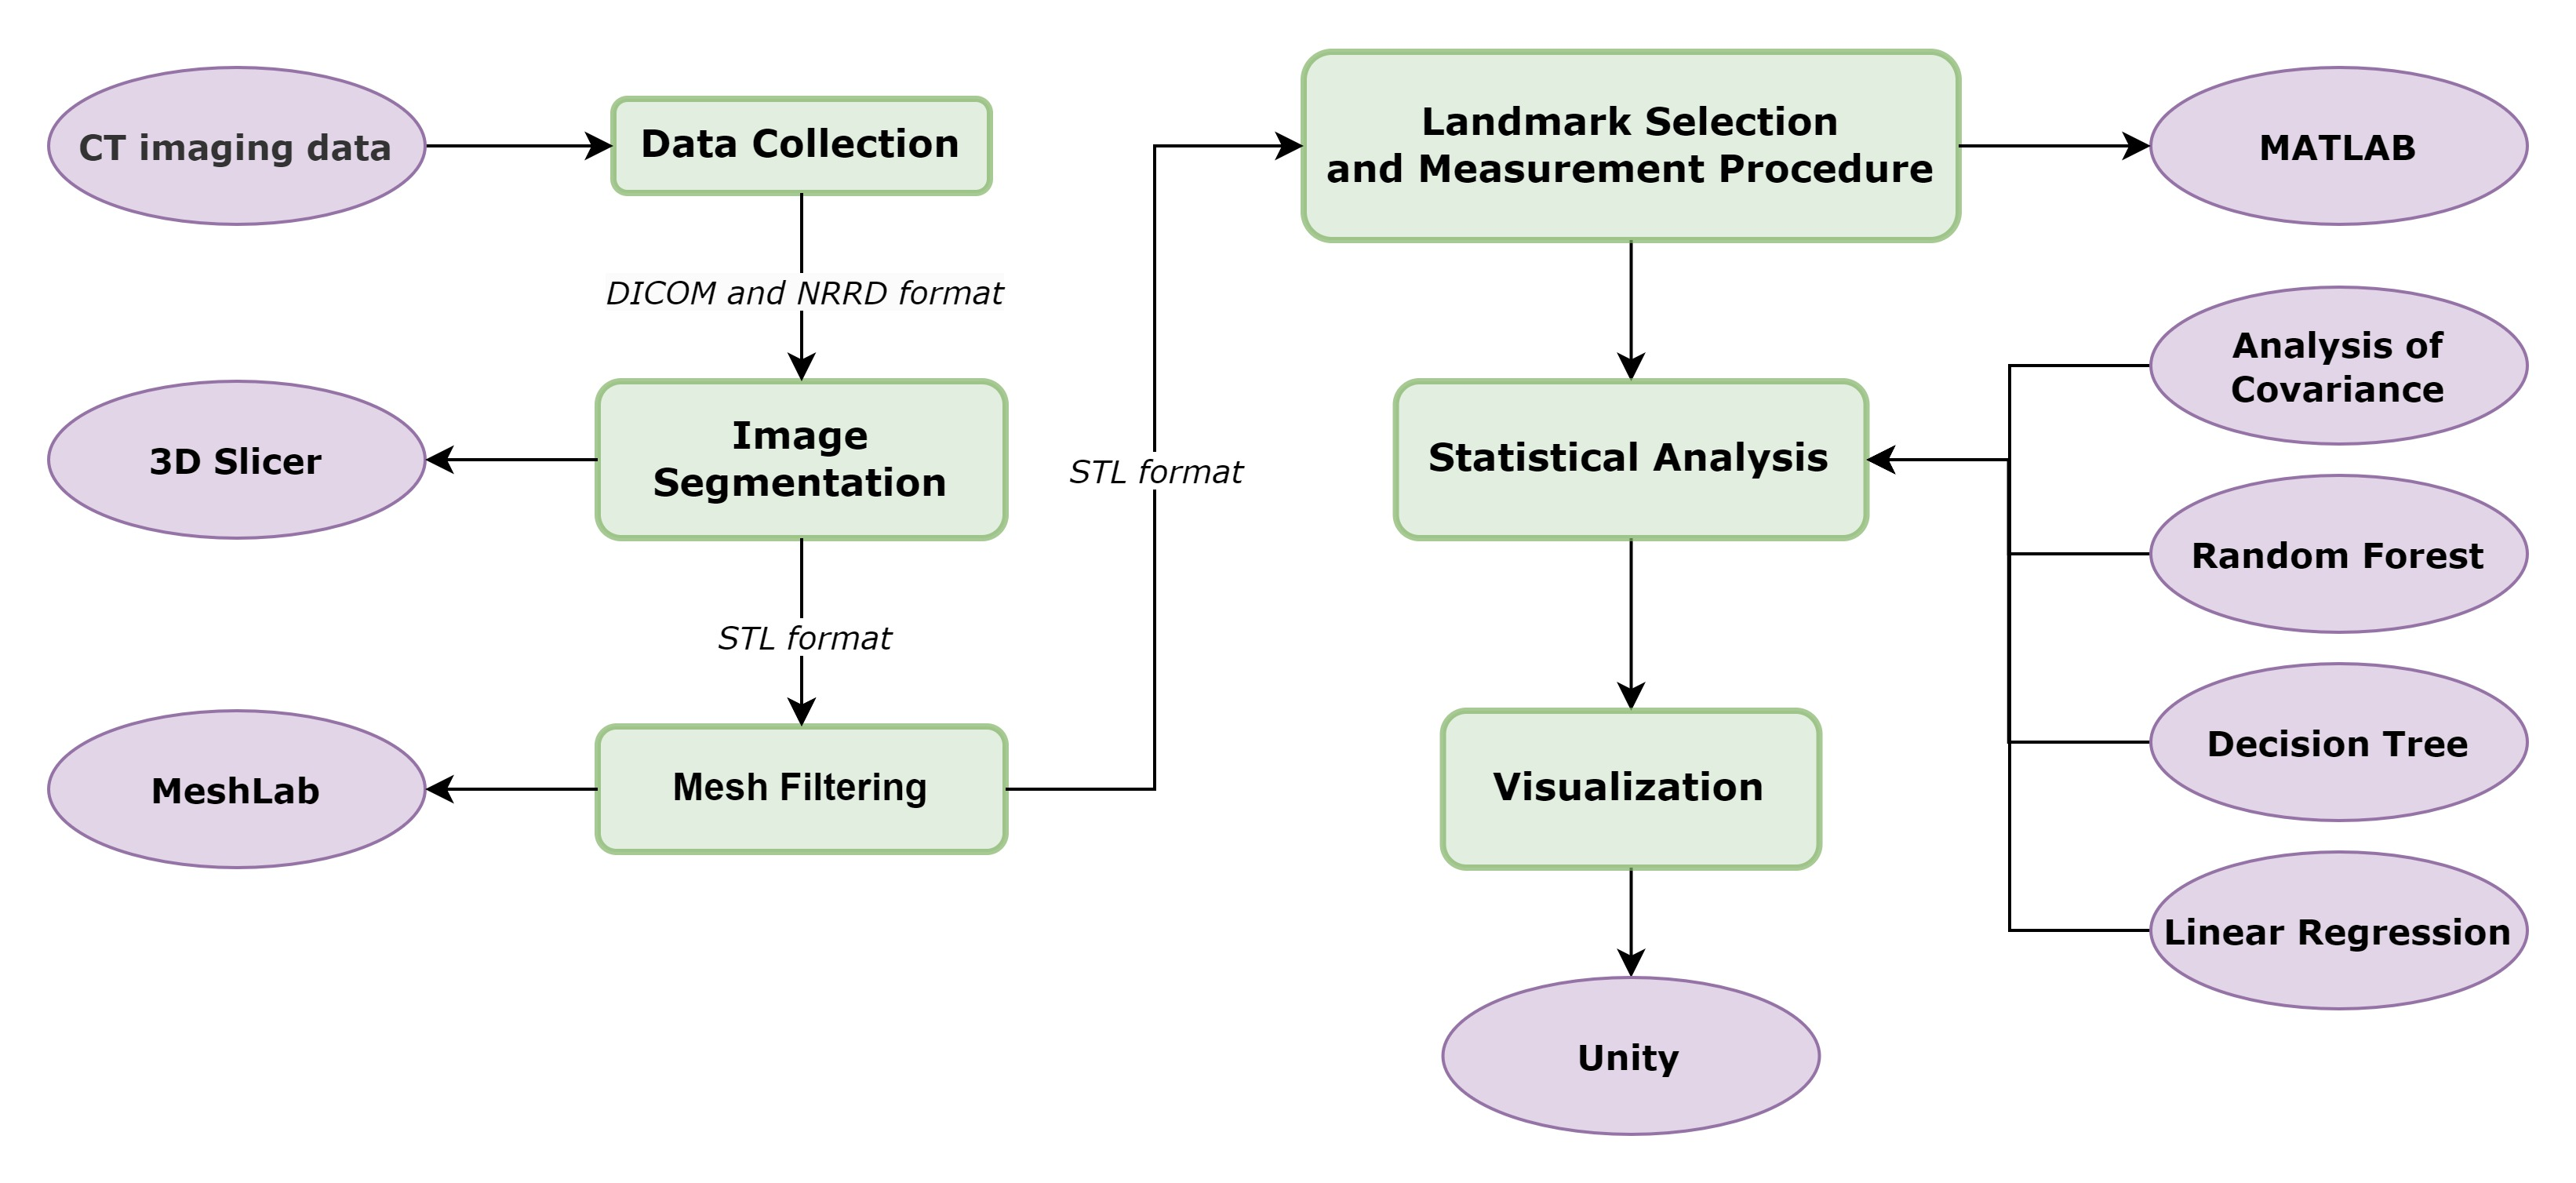
\includegraphics[width=1\linewidth]{Definitions/diagramma.jpg}
\caption{Workflow diagram}
\label{fig1}
\end{minipage}
\end{figure}

\subsection{Image Segmentation and Cleaning}

The DICOM and NRRD files taken by CBCT were 3D modeled for the patient’s hard and soft tissues using the 3DSlicer program.
\\To extract hard and soft tissues in 3D, the Hounsfield Unit (\textbf{HU}) [value, a numerical value] representing the grayscale, was adjusted in the Segmentation Editor section. 

The extracted segmentation was refined utilizing the 'Smoothing' command, which applies a Gaussian filter to smooth surfaces and reduce irregularities. Additionally, the 'Island' command was employed to manage and manipulate separate regions, keeping only the largest island.

% [Using “Smoothing” and “Islands” commands, the extracted segmentation was refined.
% The “Smoothing” command is used to smooth out the segmentation surfaces and reduce irregularities, which was particularly useful given the contained noise. The smoothing technique used was Gaussian, which applies a Gaussian filter to smooth the surfaces.\\
% “Islands” command is used to manage and manipulate separate regions within a segmentation. The operation used was “Keep largest island” which retains only the largest island and removes all others.]

Finally, the hard and soft segmentation was exported in the ‘.stl’ format for the next step.


\subsection{Mesh Filtering}

After importing the mesh in .stl format from 3DSlicer, the next step was cleaning the mesh using \textbf{MeshLab}.
For subsequent manipulation in Matlab, it was not necessary to keep the entire model but only the facial shell for both tissues, so only the frontal vertices of the models were selected using the z-painting command.

The last step in this phase was to export the final model in “.stl” format.

\subsection{Landmark Selection and Measurement Procedure}
For each patient, the further refined mesh was imported into MATLAB and the following facial landmarks were manually identified:
\begin{itemize}
    \item Glabella
    \item Nasion
    \item Orbitale (right and left)
    \item Superius (right and left)
    \item Zygion (right and left)
    \item Mid-Philtrum (A-Point)
\end{itemize}

These landmarks were chosen based on their relevance in craniofacial studies and their ease of identification on images.
\\The initial goal of the analysis was to examine additional landmarks related to the lower part of the face, but due to the presence of external objects in that area, they were removed from the analysis.

Each landmark’s FSTT was then measured and recorded for statistical analysis.

\begin{figure}[H]
\centering
\begin{minipage}{0.45\textwidth}
\centering
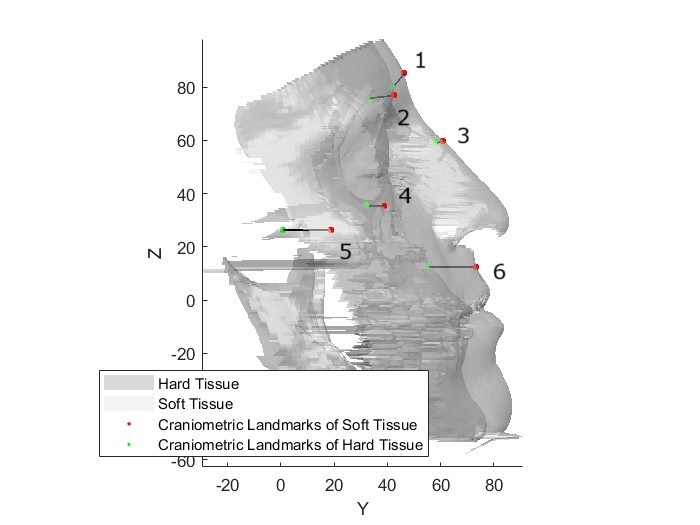
\includegraphics[width=1\linewidth]{Definitions/right_num.jpg}
\caption{Soft-tissue thickness
measurements: 1. Glabella, 2. Superius (right), 3. Rhinion, 4. Orbitale (right),  5. Zygion (right), 6. Midphiltrum (right)}
\label{fig1}
\end{minipage}\hfill
\begin{minipage}{0.45\textwidth}
\centering
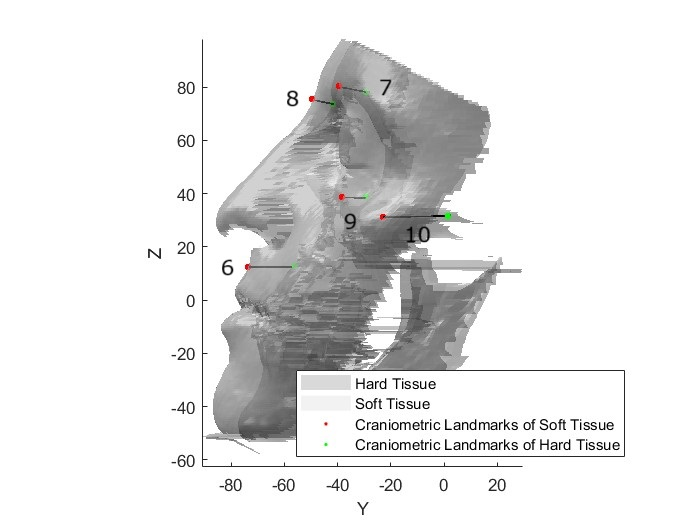
\includegraphics[width=1\linewidth]{Definitions/left_num.jpg}
\caption{Soft-tissue thickness
measurements: 6. Midphiltrum (left), 7. Superius (left), 8. Nasion, 9. Orbitale (left),  10. Zygion (left)}
\label{fig2}
\end{minipage}
\end{figure}


\subsection{Statistical Analysis} \label{sec:sez2-5}

In this last part of the analysis, the primary objective was to discern potential correlations between these measurements and variables such as \textbf{age} and \textbf{sex}, and then integrating also the \textbf{BMI} factors. 

The FSTTs of the two datasets were combined for the analysis, conducting a preliminary check for the presence of outliers and removing them to carry out a more precise analysis.

Then, several statistical and machine learning methods were employed to analyze the relationship between FSTT and variables mentioned before.

Firstly the \textbf{Pearson correlation} was used to understand the relationship between the patient’s age and sex and each landmark. 
\\These insights can be valuable for understanding which distances of these landmarks are more influential in predicting demographic factors and discovering the underlying biological relationships between these variables. They can also be useful in creating more accurate predictive models.

Then, statistical method called Analysis of Covariance (\textbf{ANCOVA}), as done in \cite{ref19} was used.\\
To support this method, three distinct range for ages were considered:
\begin{enumerate}
    \item Under 25 (<25)
    \item 25-60 (>=25 and <60)
    \item Over 60 (>=60)
\end{enumerate}

To determine the significance of these relationships, the \textbf{p-value} was examined and used to analyze the most significant landmarks (those one with p-value<0.05).\\ 

Next, a \textbf{K-fold cross-validation} was performed for both \textbf{Random Forest} (RF) and \textbf{Decision Tree} (DT) models.

The analysis began by dividing the data into training and test sets for each fold of the cross-validation process using a K value of 10. 

RF and DT were trained separately for predicting gender, age, and combined labels (age+gender), using \textit{RandomForestClassifier} class to train the RF models, and the \textit{DecisionTreeClassifier} class to train the DT models.

In addition to computing accuracy, the importance of each predictor variable in the models was also computed. This was done using the \textit{features\_importances\_} parameter for the RF models and the \textit{features\_importances\_} function for the DT models.

Given that the Head-Neck-CT dataset does not provide any information related to \textbf{BMI}, only the dataset provided by the university professors was used in the second step of the statistical analysis. This was helpful in evaluating the relationship related to this factor and analyzing how this analysis might change if integrated with more information. 
In this case, four ranges of BMI were considered:

\begin{enumerate}
    \item Underweight (<18.5)
    \item Normal weight (>=18.5 and < 24.9)
    \item Overweight (>= 24.9 and < 29.9)
    \item Obese (>=29.9)
\end{enumerate}
And 3 ranges for ages:
\begin{enumerate}
    \item Under 24 (<24)
    \item 24-29 (>=24 and <90)
    \item Over 29 (>= 29) 
\end{enumerate}

In this case, the use of \textbf{Leave-One-Out} approach for RF and DF was necessary since the dataset had only 14 patients.
 
In terms of expected results, it is anticipated to see which predictor variables are most important for each model and each type of label. There is also an expectation to see how well each model performed in terms of accuracy. 

The specific results will depend on the data and the specific settings used for the models. For instance, the number of trees in the RF models is set to 100 in this analysis, but different results could be obtained with a different number of trees. More trees lead to a more diverse set of predictions, which can result in a more stable and robust model. 
The number is set to 100 because training a RF model involves creating multiple decision trees, each of which requires computational resources. This can be helpful to ensure that the model can be trained in a reasonable amount of time without requiring excessive computational resources.

Similarly, the specific method of splitting the data into folds can also affect the results. Since the classes in data are imbalanced, due to the limited dataset used for the analysis, stratified K-Fold Cross-Validation was the better choice. It works by preserving the original distribution of classes in each fold, ensuring that the proportions between classes are conserved. This approach makes sure that each class is adequately represented across all folds, allowing for a fair and accurate evaluation of the model’s performance.

This information aids in analyzing the relationship between FSTT and variables such as age, sex, and BMI (also with the combination of those labels) and how well the models can be expected to perform on new data.

\subsection{Visualization}

As a conclusion of the work, Unity software was used for the visualization of the obtained results.

%%%%%%%%%%%%%%%%%%%%%%%%%%%%%%%%%%%%%%%%%%
\section{Results}
\label{sec:res}


\subsection*{Mean and standard deviation analysis}
The estimated average soft tissue thicknesses and the standard deviation (\textbf{std}), considering subject sex, are presented in Table \ref{tab1}. The values are thicker soft tissues for men than for women, especially for some points like \textbf{orbitals} and \textbf{zygions}.


Figure \ref{fig4} and Figure \ref{fig5} represent the trend of the average FSTT for men and women respectively, this time considering three age groups (Under 25, 25-60, Over 60). \\ From this, it seems that the thickness for some landmarks tends to increase with the rise of the age group in both sexes.\\
Considering the general trend of FSTT for men and women, it seems that the points relative to the facial medial points, therefore \textbf{glabella}, \textbf{rhinion} and \textbf{mid-philtrum}, are relatively thicker in men, regardless of the age groups considered.

However, both female and male FSTT tend to show an alternating pattern of increase and decrease with age.

\begin{table}[H]
\centering

\resizebox{0.5\linewidth}{!}{%

\begin{tabular}{cc|cccccc|} \cline{3-8}
 &  & \multicolumn{3}{c|}{Men} & \multicolumn{3}{c|}{Women} \\ \hline
\multicolumn{2}{|c|}{Landmarks} & Mean & Std & \multicolumn{1}{c|}{N} & Mean & Std & N \\ \hline
\multicolumn{2}{|c|}{Glabella} & 6.19 & 1.12 & \multicolumn{1}{c|} {36} & 5.95 & 1.10 & 20 \\ \hline
\multicolumn{2}{|c|}{Nasion} & 7.33 & 1.07 & \multicolumn{1}{c|}{32} & 7.15 & 1.38 & 20 \\\hline
\multicolumn{2}{|c|}{\begin{tabular}[c]{@{}c@{}}Orbitale\\ right\end{tabular}} & 8.52 & 2.22 & \multicolumn{1}{c|}{35} & 8.06 & 2.23 & 20 \\ \hline
\multicolumn{2}{|c|}{\begin{tabular}[c]{@{}c@{}}Orbitale \\ left\end{tabular}} & 8.53 & 2.31 & \multicolumn{1}{c|}{34} & 7.79 & 1.95 & 19 \\ \hline
\multicolumn{2}{|c|}{\begin{tabular}[c]{@{}c@{}}Orbitale superius\\ right\end{tabular}} & 8.42 & 1.61 & \multicolumn{1}{c|}{34} & 7.85 & 1.85 & 21 \\ \hline
\multicolumn{2}{|c|}{\begin{tabular}[c]{@{}c@{}}Orbitale superius\\ left\end{tabular}} & 8.24 & 1.82 & \multicolumn{1}{c|}{34} & 7.58 & 1.47 & 21 \\ \hline
\multicolumn{2}{|c|}{Zygion right} & 9.47 & 1.50 & \multicolumn{1}{c|}{32} & 9.09 & 1.14 & 20 \\ \hline
\multicolumn{2}{|c|}{Zygion left} & 9.78 & 1.85 & \multicolumn{1}{c|}{32} & 8.99 & 1.35 & 20 \\ \hline
\multicolumn{2}{|c|}{Rhinion} & 4.19 & 0.89 & \multicolumn{1}{c|}{30} & 3.97 & 1.09 & 18 \\ \hline
\multicolumn{2}{|c|}{\begin{tabular}[c]{@{}c@{}}Mid-Philtrum\\ (A-Point)\end{tabular}} & 13.99 & 2.34 & \multicolumn{1}{c|}{36} & 13.48 & 2.45 & 21 \\\hline
\end{tabular}%
}
\caption{Mean and std FSTT for men and women \label{tab1}}
\end{table}



\begin{figure}[H]
\begin{minipage}{0.5\textwidth}
\centering
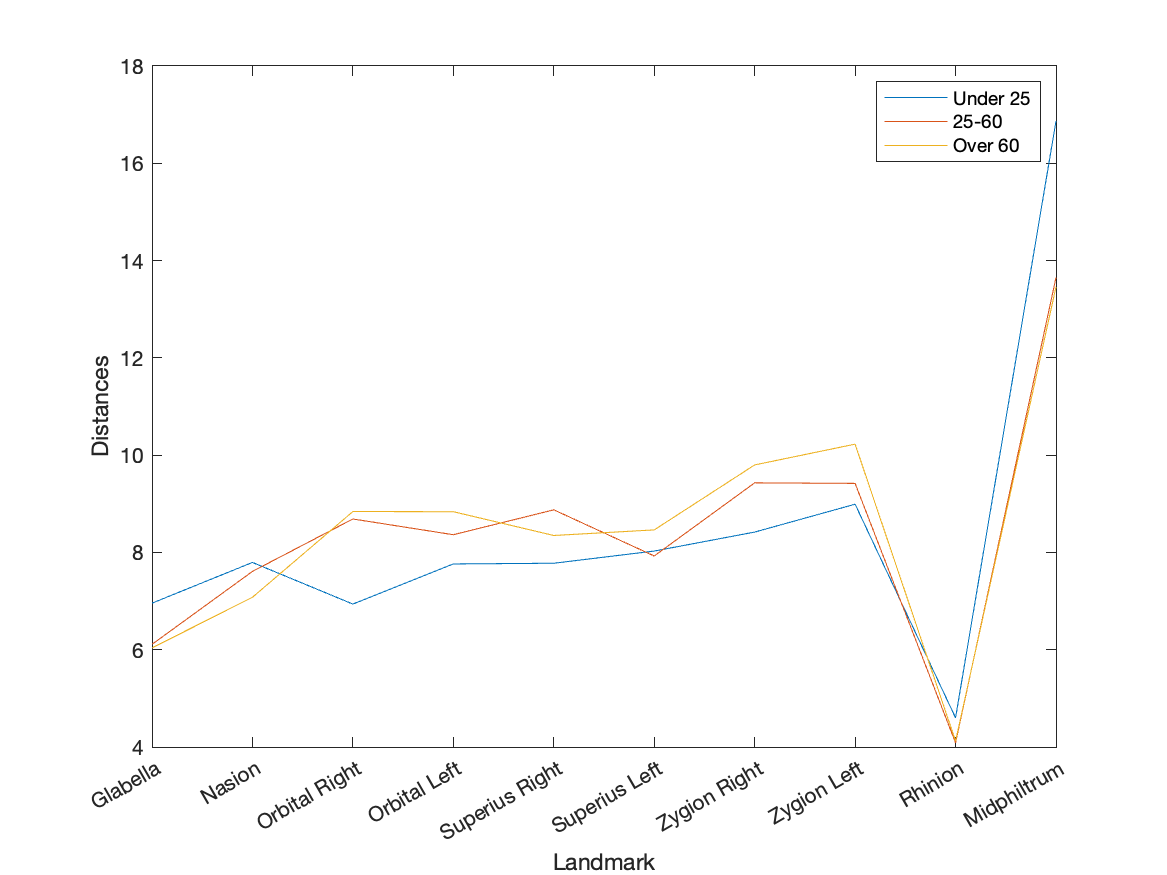
\includegraphics[width=1\linewidth]{Definitions/Men_distances_after_cleaning.png}
\caption{Mean FSTT for Men}
\label{fig4}
\end{minipage}%
\begin{minipage}{0.5\textwidth}
\centering
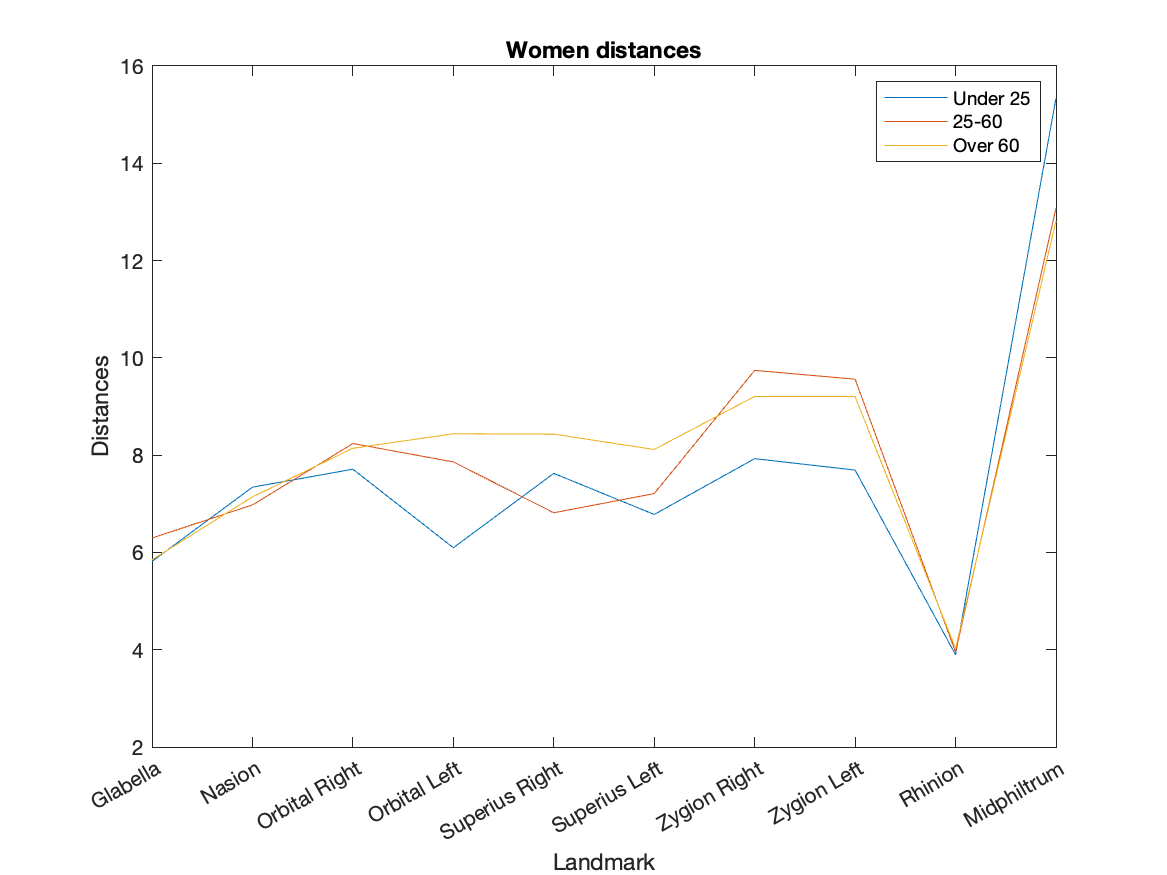
\includegraphics[width=1\linewidth]{Definitions/Women_distances_after_cleaning.png}
\caption{Mean FSTT for Women}
\label{fig5}
\end{minipage}
\end{figure}
 

\subsection*{Regression}

The linear regression models for predicting age, sex, and age bins of individuals demonstrated varying accuracy. For age prediction, the model achieved an overall accuracy of \textbf{0.96}, indicating \textbf{high precision, recall, and F1-scores} across age groups. Notably, precision, recall, and F1-scores were \textbf{perfect for the 51-60 and 80+ age groups}. The sex prediction model attained \textbf{perfect accuracy (1.00)} using all landmarks but showed \textbf{decreased accuracy (0.75)} when considering individual patient landmarks, particularly for class female, where precision, recall, and F1-score dropped to 0.00. The age bin prediction model had an overall accuracy of \textbf{0.67}, performing moderately for the 61-70 age group but poorly for other age groups. These results indicate that the models are \textbf{highly effective for predicting age and sex when considering all landmarks} but exhibit decreased performance with individual landmarks or when predicting age bins.

\subsection*{Pearson correlation} \label{subsec:pearson-correlation}
In the analysis conducted with \textbf{Pearson correlation}, also considered in \cite{ref19}, the results of which are presented in Table \ref{tab3}, each landmark has corresponding numerical values indicating its correlation with age, gender M (presumably male), and gender F (presumably female). 

For instance, for age correlation \textbf{glabella} and \textbf{rhinion} seem to have the highest positive correlation , while most of the landmarks have relatively low correlations.

For gender correlation, \textbf{mid-philtrum}, \textbf{rhinion} and \textbf{nasion} have the highest correlation for male (and lowest correlation for female).


\begin{table}[H]
\centering
\begin{minipage}{0.45\textwidth}
\centering
\resizebox{\linewidth}{!}{%
\begin{tabular}{clccc}
\hline
\multicolumn{2}{c}{} & \multicolumn{3}{c}{Correlation} \\\hline
\multicolumn{2}{c}{Landmarks} & Age & Gender\_M & Gender\_F \\ \hline
\multicolumn{2}{c|}{Glabella} & 0.159 & 0.186 & -0.186 \\\hline 
\multicolumn{2}{c|}{Nasion} & 0.049 & 0.224 & -0.224 \\ \hline
\multicolumn{2}{c|}{\begin{tabular}[c]{@{}c@{}}Orbitale\\ \end{tabular}} & 0.111 & -0.199 & 0.199 \\ \hline
\multicolumn{2}{c|}{\begin{tabular}[c]{@{}c@{}}Orbitale superius\\ \end{tabular}} & 0.103 & 0.139 & -0.139 \\ \hline

\multicolumn{2}{c|}{Zygion} & 0.020 & 0.164 & -0.164 \\ \hline

\multicolumn{2}{c|}{Rhinion} & 0.170 & 0.233 & -0.233 \\ \hline
\multicolumn{2}{c|}{\begin{tabular}[c]{@{}c@{}}Mid-Philtrum\\ (A-Point)\end{tabular}} & -0.028 & 0.361 & -0.361 \\\hline
\end{tabular}%
}
\caption{Pearson Correlation \label{tab3}}
\end{minipage}\hfill
\begin{minipage}{0.45\textwidth}
\centering
\resizebox{\linewidth}{!}{%
\begin{tabular}{clccc}
\hline
\multicolumn{2}{c}{} & \multicolumn{3}{c}{p\_values} \\ \hline
\multicolumn{2}{c|}{Landmarks} & Gender & Age & Gender+Age \\ \hline
\multicolumn{2}{c|}{Glabella} & 0.371 & 0.510 & 0.332 \\ \hline
\multicolumn{2}{c|}{Nasion} & 0.368 & 0.683 & 0.773 \\ \hline
\multicolumn{2}{c|}{Orbitale right} & 0.599 & 0.323 & 0.675 \\ \hline
\multicolumn{2}{c|}{Orbitale left} & 0.298 & 0.165 & 0.749 \\ \hline
\multicolumn{2}{c|}{\begin{tabular}[c]{@{}c@{}}Orbitale superius\\ right\end{tabular}} & 0.277 & 0.619 & 0.164 \\ \hline
\multicolumn{2}{c|}{\begin{tabular}[c]{@{}c@{}}Orbitale superius\\ left\end{tabular}} & 0.202 & 0.281 & 0.771 \\ \hline
\multicolumn{2}{c|}{Zygion right} & 0.223 & {\color[HTML]{FE0000} 0.010} & 0.814 \\ \hline
\multicolumn{2}{c|}{Zygion left} & 0.169 & 0.132 & 0.528 \\ \hline
\multicolumn{2}{c|}{Rhinion} & 0.09 & 0.369 & 0.420 \\ \hline
\multicolumn{2}{c|}{\begin{tabular}[c]{@{}c@{}}Mid-philtrum\\ (A-Point)\end{tabular}} & 0.193 & {\color[HTML]{FE0000} 0.001} & 0.839 \\ \hline
\end{tabular}%
}
\caption{P-value for ANCOVA analysis \label{tab4}}
\end{minipage}
\end{table}

\subsection*{ANCOVA and RF analysis} \label{subsec:ancova-rf-analysis}

Subsequently, the \textbf{ANCOVA} statistical analysis was performed, collecting the results in a Table \ref{tab4}. The p value was considered statistically significant when \textbf{p\_values <0.05}. By analyzing the obtained results, it is possible to state that only for the age analysis there is a significant value, both for the \textbf{right zygion} and the \textbf{mid-philtrum}.

The latest analysis, which took into account the age and sex of the patients, used two classification models, RF and DT. 

Only the results related to the most performant model (RF) were reported in the Figure {\ref{fig:fig6}}. \\ The analysis conducted allowed us to examine which landmarks (considering their thicknesses) had the most influence in the classification of age, gender, and then in age and gender combined together. 

As can be seen from the figures, considering only gender, the 3 most significant landmarks turn out to be \textbf{nasion}, \textbf{superius right} and \textbf{zygion right}. 
Considering only age, the top-3 landmarks turn out to be \textbf{orbital right}, \textbf{orbital left} and \textbf{mid-philtum}.
Considering the combination between gender and age, the top-3 landmarks turn out to be \textbf{orbital left}, \textbf{zygion right} and \textbf{mid-philtum}.

\begin{figure}[H]
    \centering
    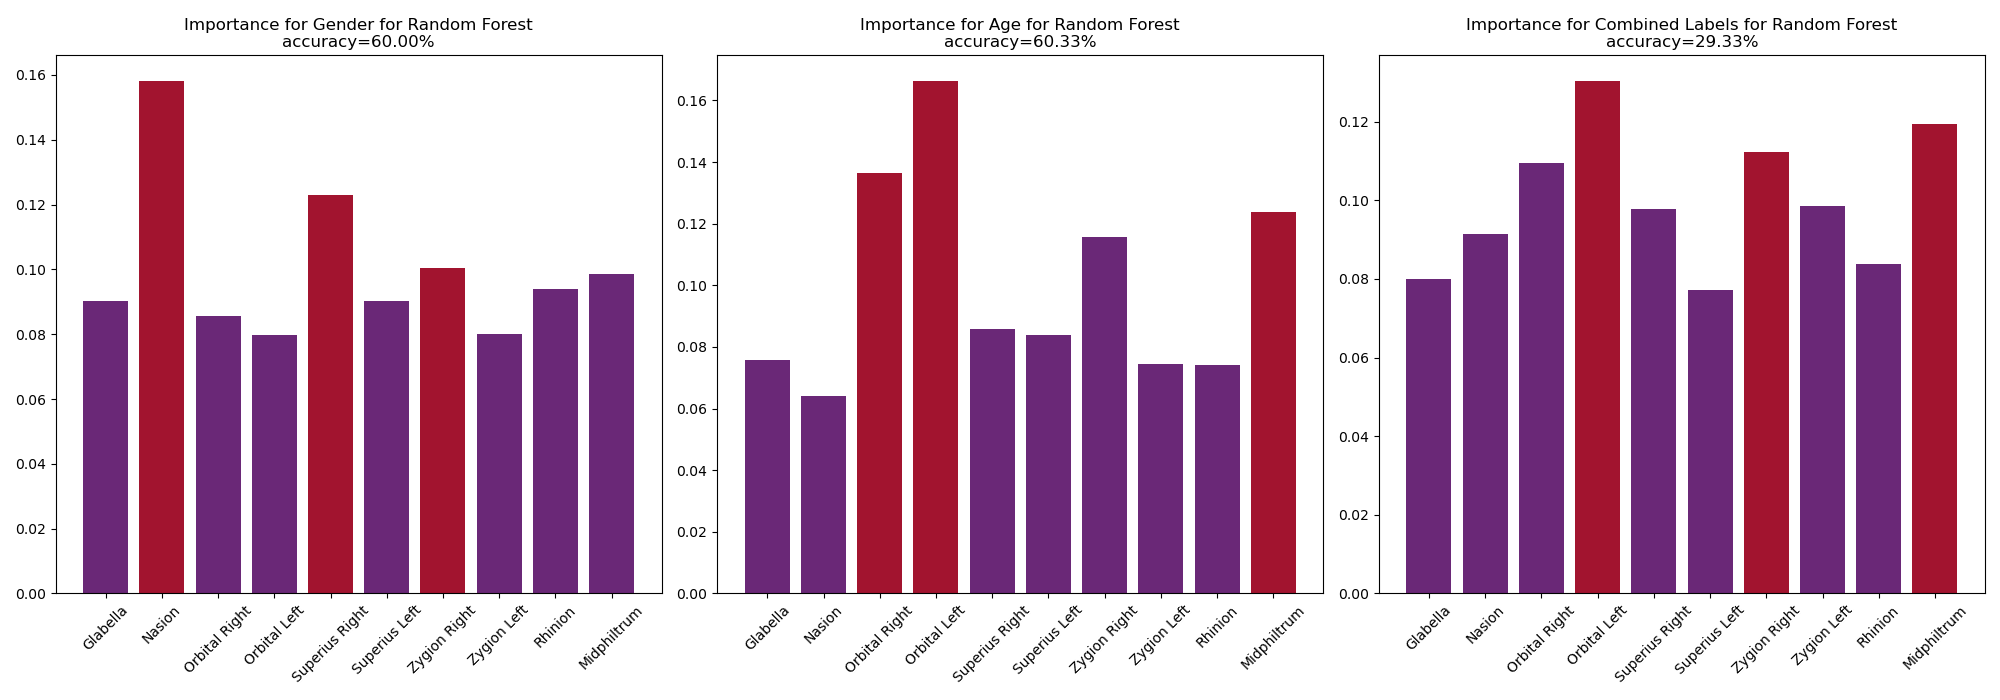
\includegraphics[width=1\linewidth]{Definitions/RF_analysis.png}
    \caption{RF analysis}
    \label{fig:fig6}
\end{figure}

Given that the first analysis only considered sex and age, since the Head-Neck-CT dataset does not contain information related to BMI, in this last phase an analysis was conducted only on the dataset provided by Professor Olivetti and Professor Marcolin, also considering the BMI factor and repeating the same statistical analysis steps described previously. 

From the analysis of the dataset, it emerged that, considering age ranges, not all weight categories were covered. For this reason, the behavior of the average FSTT for the different bands of age and BMI was not analyzed, as the result was not complete enough to be included in the analysis. 
Considering the BMI factor and distinguishing the patients as male or female, the trend described in the figure was obtained.
From this figure, it can be noted that as the weight category increases, the values of the FSTT tend to be thicker. For example, the zygion and the midphiltrum seem to have significant increases for men, while for women the increase seems to also cover the orbitals and the median points of the face.


\begin{figure}[H]
    \begin{minipage}{0.45\textwidth}
        \centering
        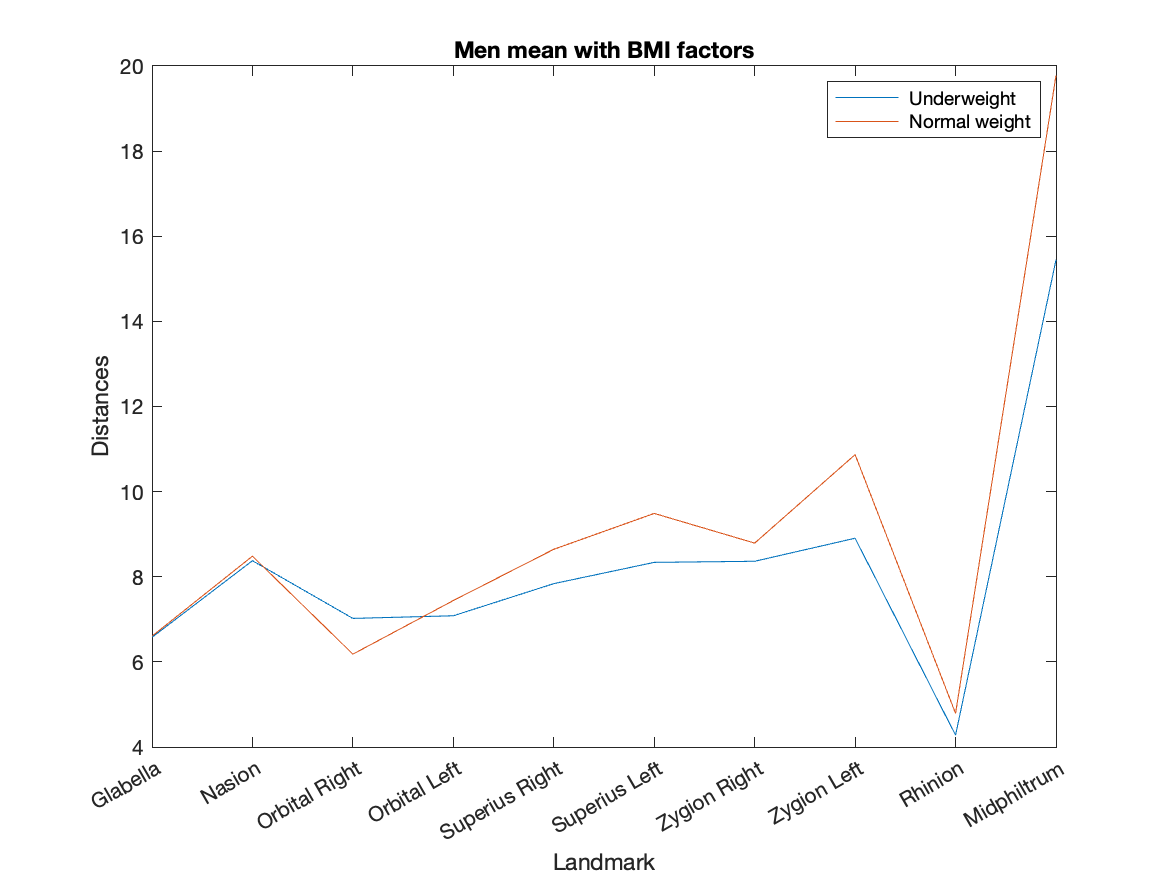
\includegraphics[width=\linewidth]{Definitions/Men_mean_BMI_withoutAge.png}
        \caption{Men mean considering BMI ranges}
        \label{fig:fig7}
    \end{minipage}
    \hfill
    \begin{minipage}{0.45\textwidth}
        \centering
        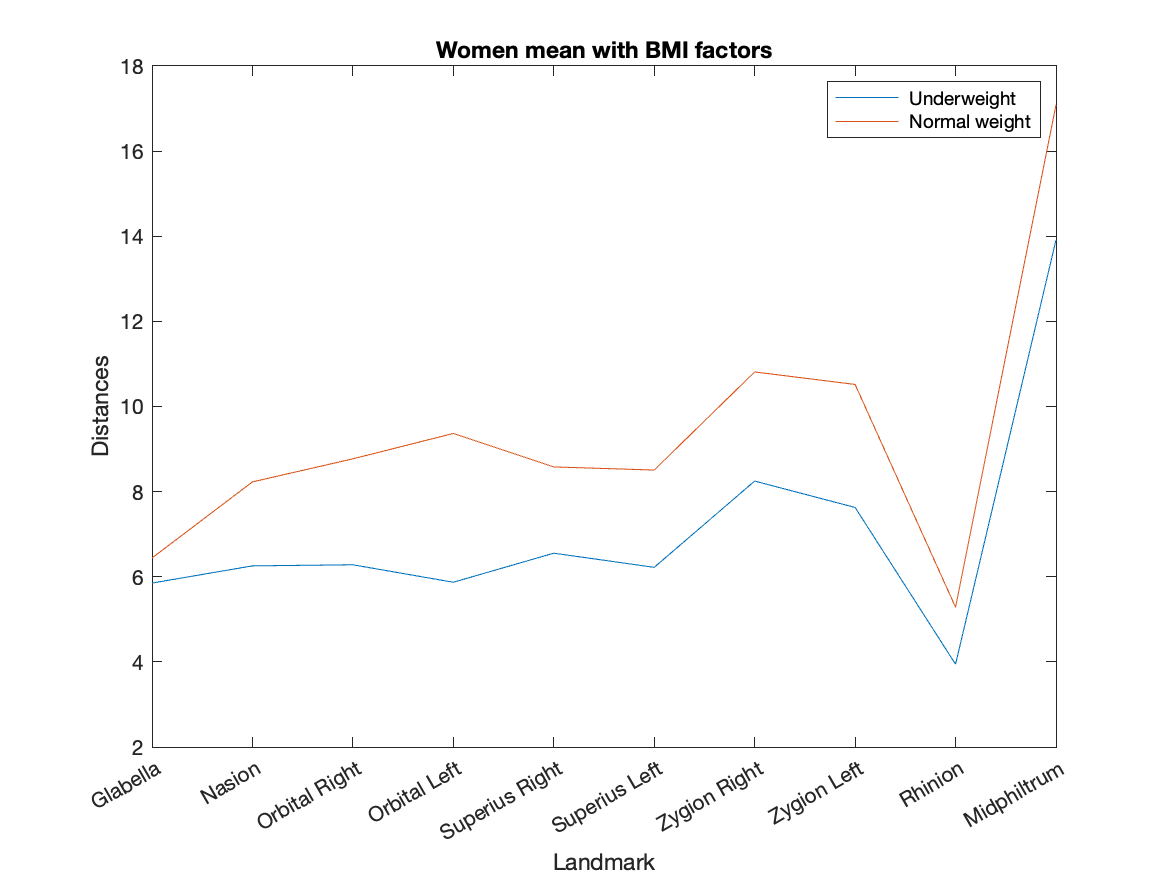
\includegraphics[width=\linewidth]{Definitions/Women_mean_BMI_withoutAge.png}
        \caption{Women mean considering BMI ranges}
        \label{fig:fig8}
    \end{minipage}
\end{figure}


Using ANCOVA analysis, the results obtained are represented in Figure \ref{fig:fig9} and cover the analysis by gender, age, BMI, the interaction between gender and BMI (\textbf{Interaction GB}), the interaction between gender and age (\textbf{Interaction GA}), the interaction between age and BMI (\textbf{Interaction AB}) and finally the interaction between gender,age and BMI combined (\textbf{Interaction GAB}).

By observing this plot, it is possible to notice how the addition of the BMI factor could improve the analysis and provide more accurate results. Based on these results, it would seem that the landmarks that have the most influence are:
\begin{enumerate}
    \item Glabella, for the Interaction GAB
    \item Nasion, for the BMI, Interaction AB, and Interaction GAB analysis
    \item Superius Left, for gender, BMI, Interaction GB, Interaction AB and Interaction GAB analysis 
    \item Zygion Left, for BMI, Interacion GB, Interaction AB and Interaction GAB analysis
    \item Rhinion, for gender, BMI and Interaction GB analysis

\end{enumerate}


\begin{figure}[H]
    \centering
    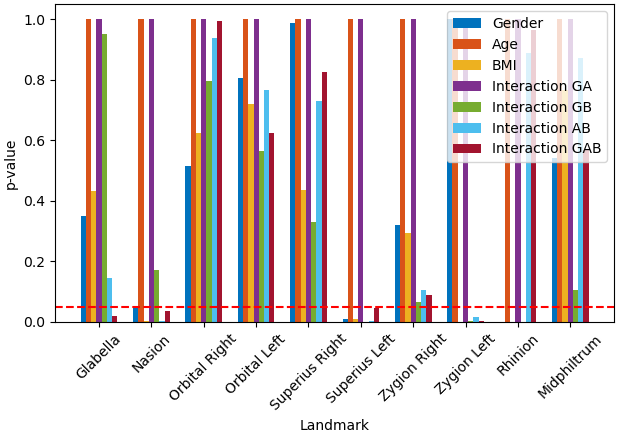
\includegraphics[width=0.6\linewidth]{Definitions/ANCOVA_BMI_after_cleaning.png}
    \caption{ANCOVA analysis with BMI factor}
    \label{fig:fig9}
\end{figure}

Subsequently, the RF model was used, obtaining the results shown in Figure \ref{fig:fig10}.

As can be seen from the figures, considering only BMI, the 3 most significant landmarks turn out to be \textbf{nasion}, \textbf{superius right} and \textbf{superius left}. 
Considering age and BMI combined, the top-3 landmarks turn out to be \textbf{glabella}, \textbf{nasion} and \textbf{superius left}.
Considering the combination between gender and BMI, the top-3 landmarks turn out to be \textbf{nasion}, \textbf{superius right} and \textbf{superius left}.
Lastly, in the interaction between gender, age and BMI, the 3 most significant landmarks turn out to be \textbf{nasion}, \textbf{superius right} and \textbf{zygion right}.

\begin{figure}[H]
    \centering
    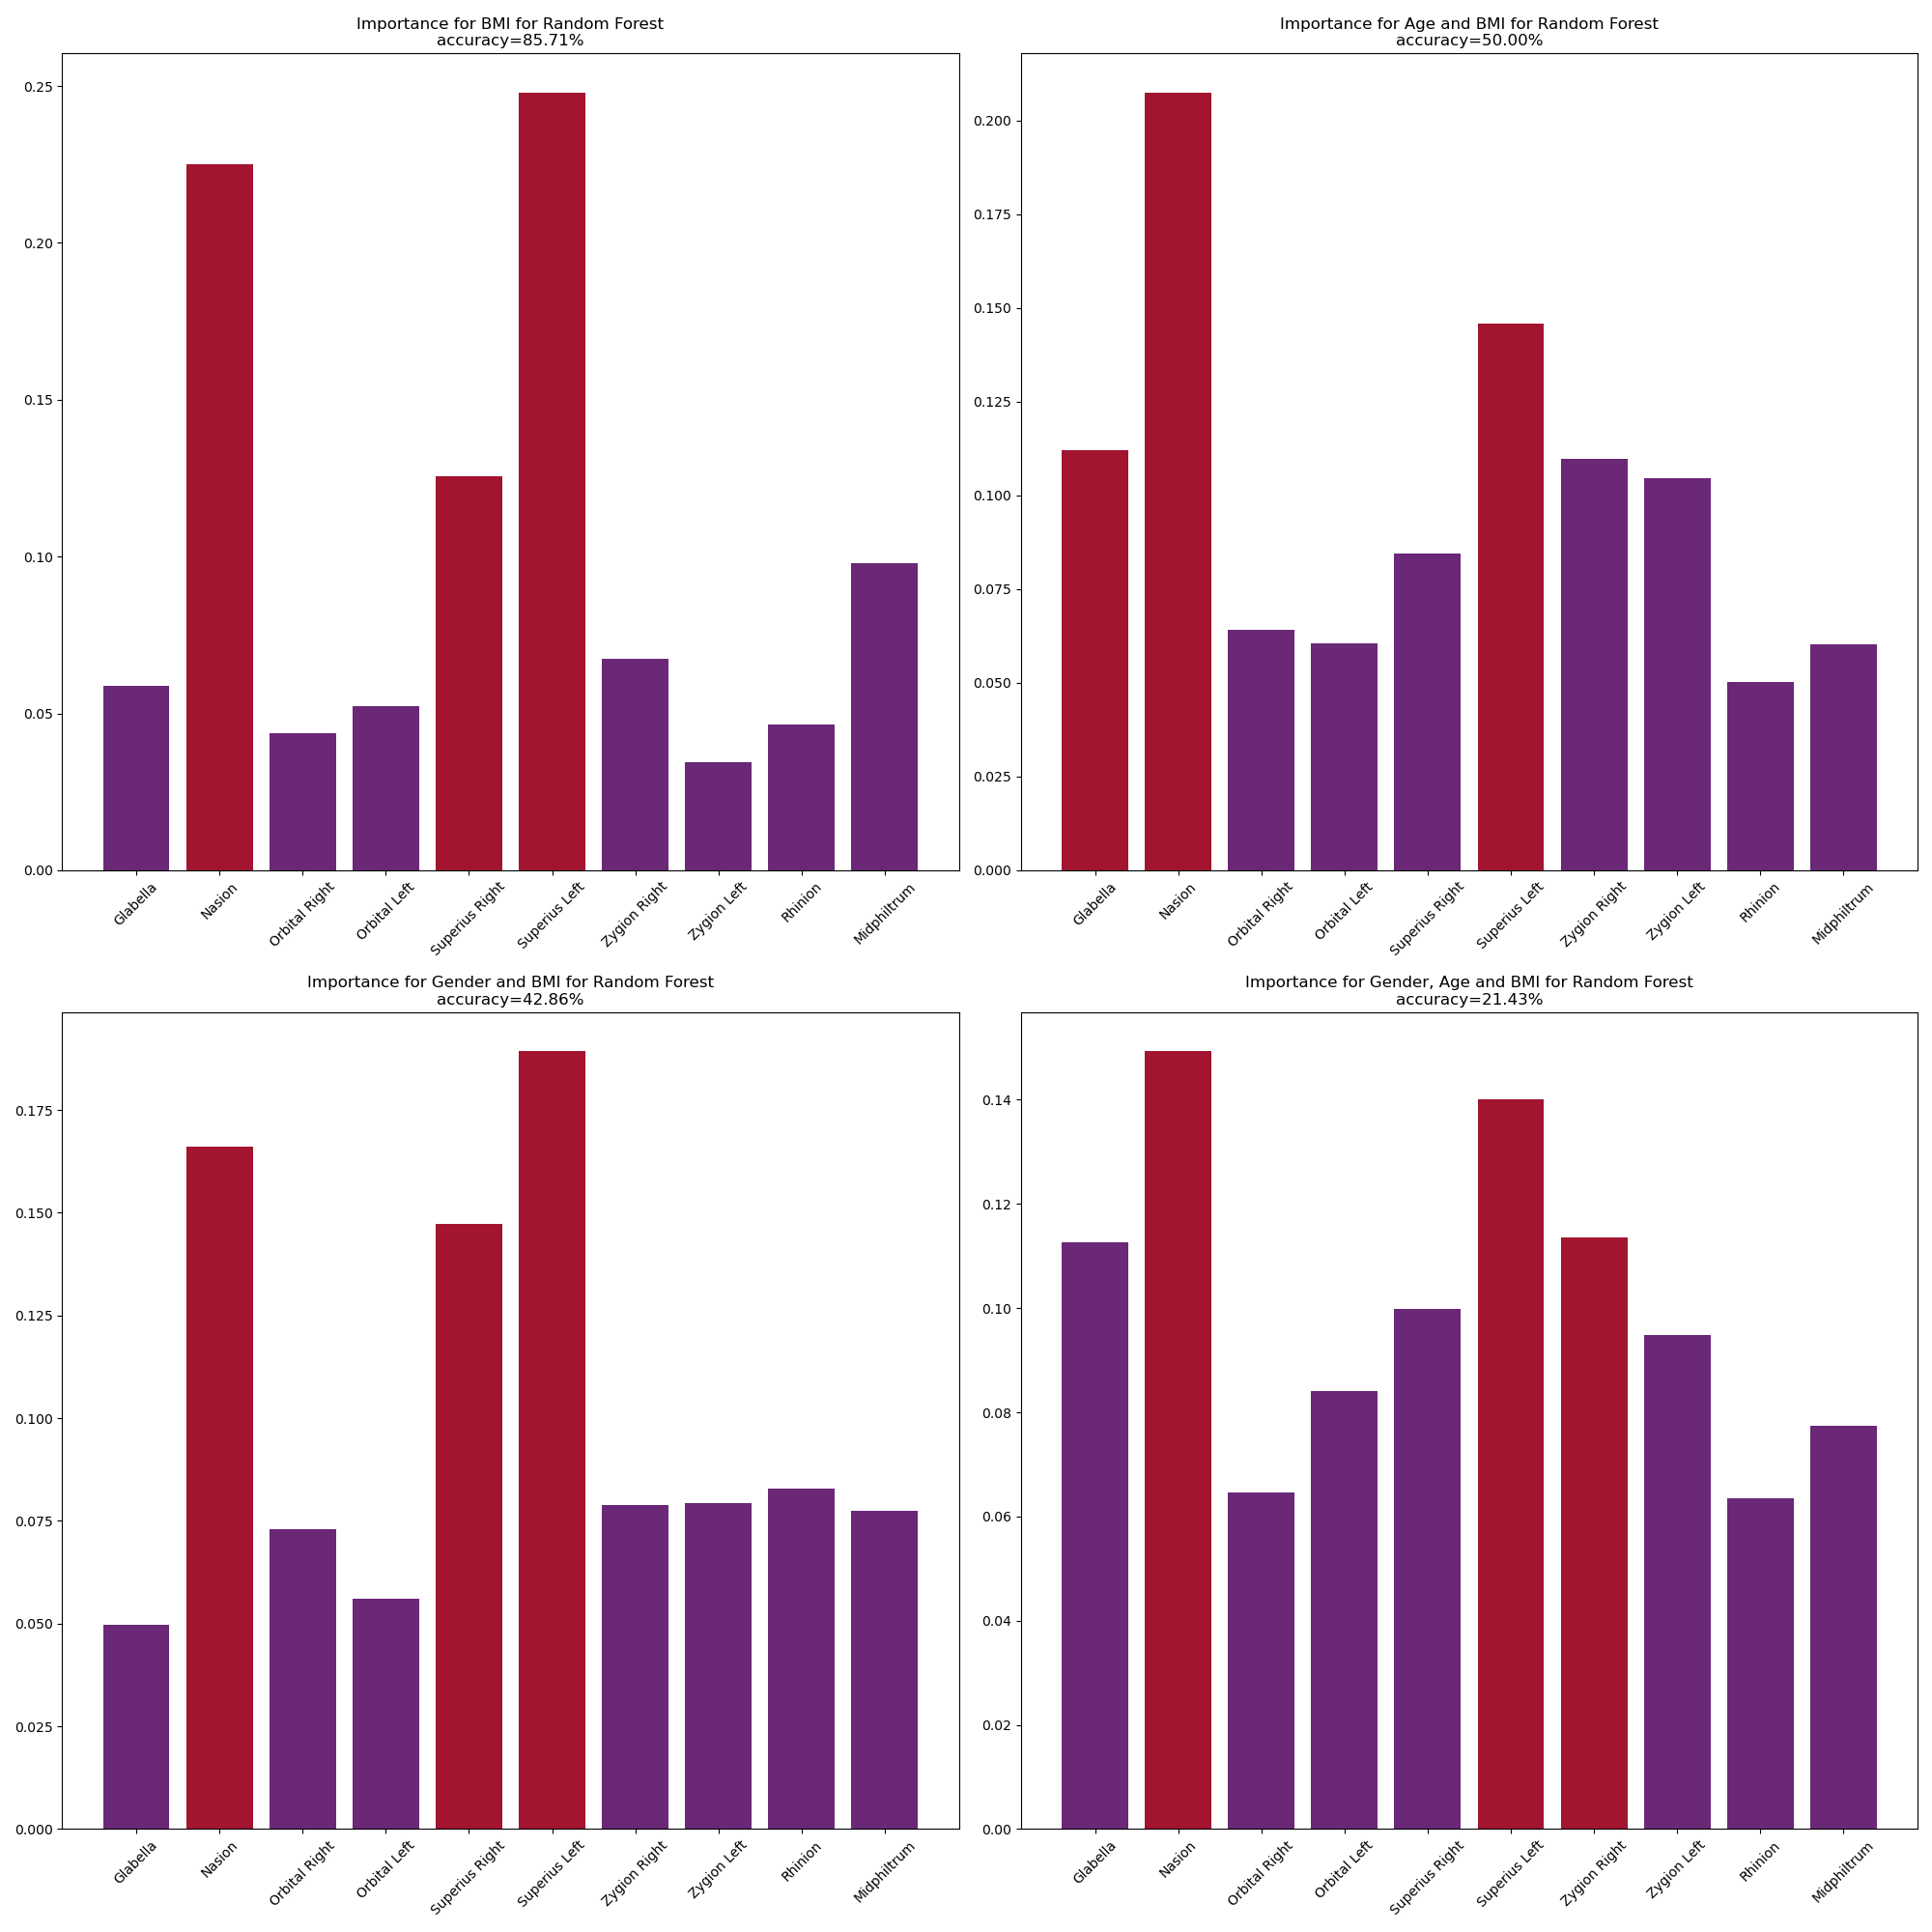
\includegraphics[width=0.75\linewidth]{Definitions/rf_bmi.png}
    \caption{RF analysis with BMI factor}
    \label{fig:fig10}
\end{figure}

%%%%%%%%%%%%%%%%%%%%%%%%%%%%%%%%%%%%%%%%%%
\section{Discussion}
\label{sec:disc}

Findings of this study provide significant insights into the influence of demographic factors on FSTT, with potential applications in FFR and related fields. 
% These results indicate that BMI plays a crucial role in determining FSTT and suggest that, with a more in-depth analysis for the weight categories missing in this analysis, it could confirm the existing literature that highlights the relationship between a higher BMI and increased tissue thickness at various craniofacial reference points. Specifically, data are aligned with the findings of Piombino et al. \cite{ref19}, who also noted significant correlations between BMI and FSTT, particularly in the orbitals and zygions regions \cite{ref1,ref2}.

Comparative analysis with previous studies reveals both similarities and differences. For instance, this study's observation of marginal impacts of age and sex on FSTT concurs with Piombino et al. \cite{ref19}, yet contrasts with other works that reported more pronounced age-related changes in FSTT (e.g., Codinha et al. \cite{ref13}) \cite{ref1,ref13}. Such discrepancies could stem from methodological differences, including the source and type of imaging data and demographic variations among study populations.

Table \ref{tab1} compares the FSTT averages with the main papers used and cited in this analysis, highlighting how it is plausible to state that the thickness for some landmarks is greater for men than for women. \\ Regarding the trend of FSTT averages for each age group, thicknesses tend to increase with age, probably due to the variation in weight distribution as the person grows. However, by expanding this analysis with a larger number of patients, it is expected that with advancing age, the FSTT tend to decrease in thickness.

Regression model for predicting age, sex, and age bins using FSTT measurements demonstrated varying levels of performance. The age prediction model achieved high accuracy, highlighting the potential of FSTT data for reliable age estimation. The sex prediction model showed perfect accuracy with all landmarks but decreased performance with individual landmarks, emphasizing the importance of comprehensive landmark analysis. Age bin prediction model showed limited accuracy, indicating challenges in categorizing individuals into specific age groups based on FSTT alone. These findings underscore the need for considering multiple demographic factors and comprehensive landmark data to enhance predictive accuracy in forensic and medical applications. 

As discussed in Section \ref{subsec:pearson-correlation}, the \textbf{Pearson correlation} highlighted how, for the correlation with age, glabella and rhinion are the landmarks with the highest positive correlation, indicating that as age increases, these thicknesses should increase. For gender correlation, mid-philtrum, rhinion and nasion have the highest correlation for male (and lowest correlation for female), suggesting that these areas of the face may be more influenced by gender. These results are consistent with what has also been stated in other papers, such as Piombino et al \cite{ref19}. 

\textbf{ANCOVA} statistical analysis shows that age has a significant impact on the thickness of the right zygion and the mid-philtrum. This suggests that these landmarks could be useful indicators of age in future studies. Results are partially confirmed when compared with previous studies, such as that of Moritsugui et al \cite{ref26}, where both rhinion and zygion right landmarks have a significant p-value. Differences, however, could be justified by the small number of initial data and the manual selection of landmarks on the meshes, which could have affected the precision of the average FSTT obtained. 

\textbf{RF} analysis identified different sets of influential landmarks for gender, age, and their combination. This suggests that the physical characteristics associated with age and gender are distinct, but there may be some overlap. For instance, the orbital left and mid-philtrum are influential for both age and the combination of age and gender. The fact that different landmarks are influential for gender and age could suggest that these characteristics develop differently and at different rates. This could have implications for understanding the development of facial traits.

Combination of age and gender seems to be best represented by the orbital left, zygion right, and mid-philtrum. This could suggest that these landmarks capture the most variance when both age and gender are considered. However, due to the low accuracy obtained for this latter consideration, this result cannot be considered significant.

This analysis was expanded to include the \textbf{BMI} factor. This addition of BMI to the ANCOVA analysis seems to have improved the accuracy of the results, providing a more comprehensive understanding of the influential landmarks.

Landmarks that stood out in this analysis showed significant influence in different interactions. For instance, glabella was influential for Interaction GAB, while nasion was influential for BMI, Interaction AB and for Interaction GAB.

This \textbf{RF} model further confirmed the importance of these landmarks. 
The findings presented in Section \ref{subsec:ancova-rf-analysis} highlight the importance of including BMI in the analysis to gain a more detailed understanding of influential landmarks. However, these conclusions are specific to the dataset and analysis methods used in this study, and additional research is necessary for validation and further exploration. A more comprehensive analysis, particularly of the missing weight categories, could reinforce existing literature on the correlation between higher BMI and increased tissue thickness at various craniofacial reference points. This study's data aligns with Piombino et al.'s findings \cite{ref19}, which also observed significant correlations between BMI and FSTT, especially in the orbitals and zygions regions \cite{ref1,ref2}.
% Results reported in Section \ref{subsec:ancova-rf-analysis} suggest that the inclusion of BMI in the analysis could provide a more nuanced understanding of the influential landmarks. However, it's important to note that these findings are based on the specific dataset and analysis methods used in this study. Further research may be needed to confirm these findings and explore their implications.

% These results indicate that BMI plays a crucial role in determining FSTT and suggest that, with a more in-depth analysis for the weight categories missing in this analysis, it could confirm the existing literature that highlights the relationship between a higher BMI and increased tissue thickness at various craniofacial reference points. Specifically, data are aligned with the findings of Piombino et al. \cite{ref19}, who also noted significant correlations between BMI and FSTT, particularly in the orbitals and zygions regions \cite{ref1,ref2}.


The primary contribution of this research resides in its comprehensive approach to the evaluation of FSTT using high-resolution DICOM data and advanced statistical and machine learning techniques. \\The study’s robustness is enhanced by integrating multiple datasets and applying stratified K-fold cross-validation.

However, this study is not without limitations. The relatively small sample size, particularly for the dataset provided by university professors, may limit the generalizability of the results. Additionally, the exclusion of lower facial landmarks due to the presence of external objects in the images restricts the comprehensiveness of the analysis.

One of the notable improvements in this study is the detailed analysis of FSTT variations based on demographic factors. This provides a more nuanced understanding compared to previous works. It enables a more accurate and personalized FFR, ultimately improving identification accuracy in forensic investigations.

The findings also have implications for maxillofacial and aesthetic surgery, aiding in surgical planning and outcome prediction.
% In the field of maxillofacial and aesthetic surgery, understanding the variations in FSTT can be crucial for predicting surgical outcomes. The facial features are defined by the distribution and volume of soft tissues, and these results can assist in planning surgeries to achieve more natural and satisfactory results. By incorporating individual demographic characteristics into surgical planning, medical professionals can better anticipate changes in facial contours post-surgery, leading to improved patient outcomes and satisfaction.
%Specifically, the development of predictive models for maxillofacial and aesthetic surgeries based on FSTT data could revolutionize pre-operative planning and lead to more personalized and precise interventions.

Future research should aim to expand the dataset, incorporating more diverse population groups and additional landmarks to provide a holistic view of FSTT variations. Advancements in imaging techniques and machine learning algorithms will further enhance the accuracy and applicability of FSTT measurements. Furthermore, exploring the integration of FSTT data with other biometric parameters could open new avenues for improving FFR and related applications. 



% This study significantly advances the understanding of FSTT variations and their implications, providing valuable insights for forensic and medical applications. Continued research and methodological improvements will further solidify the utility of FSTT in accurate and reliable FFRs and in enhancing surgical outcomes in maxillofacial and aesthetic procedures.



\begin{table}[H]
\centering

\begin{adjustwidth}{-\extralength}{0cm}

\resizebox{\linewidth}{!}{%
\begin{tabular}{ccccccccccccc}


\hline
 &  & Landmarks & Glabella & Nasion & Orbitale right & Orbitale left & \begin{tabular}[c]{@{}c@{}}Orbitale superius \\ right\end{tabular} & \begin{tabular}[c]{@{}c@{}}Orbitale superius \\ left\end{tabular} & Zygion right & Zygion left & Rhinion & \begin{tabular}[c]{@{}c@{}}Mid-philtrum\\ (A-point)\end{tabular} \\ \hline
 &  & n & 36 & 32 & 35 & 34 & 34 & 34 & 32 & 32 & 30 & 36 \\ \cline{3-13} 
 &  & {\color[HTML]{3531FF} mean} & {\color[HTML]{3531FF} 6.19} & {\color[HTML]{3531FF} 7.33} & {\color[HTML]{3531FF} 8.52} & {\color[HTML]{3531FF} 8.53} & {\color[HTML]{3531FF} 8.42} & {\color[HTML]{3531FF} 8.24} & {\color[HTML]{3531FF} 9.47} & {\color[HTML]{3531FF} 9.78} & {\color[HTML]{3531FF} 4.19} & {\color[HTML]{3531FF} 13.99} \\ \cline{3-13} 
 & \multirow{-3}{*}{M} & std & 1.12 & 1.07 & 2.22 & 2.31 & 1.61 & 1.82 & 1.50 & 1.85 & 0.89 & 2.34 \\ \cline{2-13} 
 &  & n & 20 & 20 & 20 & 19 & 21 & 21 & 20 & 20 & 18 & 21 \\ \cline{3-13} 
 &  & {\color[HTML]{FE0000} mean} & {\color[HTML]{FE0000} 5.95} & {\color[HTML]{FE0000} 7.15} & {\color[HTML]{FE0000} 8.06} & {\color[HTML]{FE0000} 7.79} & {\color[HTML]{FE0000} 7.85} & {\color[HTML]{FE0000} 7.58} & {\color[HTML]{FE0000} 9.09} & {\color[HTML]{FE0000} 8.99} & {\color[HTML]{FE0000} 3.97} & {\color[HTML]{FE0000} 13.48} \\ \cline{3-13} 
\multirow{-6}{*}{This paper} & \multirow{-3}{*}{W} & std & 1.10 & 1.38 & 2.23 & 1.95 & 1.85 & 1.47 & 1.14 & 1.35 & 1.09 & 2.45 \\ \hline
 &  & n & 13 & 13 & - & - & - & - & 13 & 13 & 13 & 13 \\ \cline{3-13} 
 &  & {\color[HTML]{3531FF} mean} & {\color[HTML]{3531FF} 6.69} & {\color[HTML]{3531FF} 6.69} & {\color[HTML]{3531FF} -} & {\color[HTML]{3531FF} -} & {\color[HTML]{3531FF} -} & {\color[HTML]{3531FF} -} & {\color[HTML]{3531FF} 10.88} & {\color[HTML]{3531FF} 10.88} & {\color[HTML]{3531FF} 3.04} & {\color[HTML]{3531FF} 10.15} \\ \cline{3-13} 
 & \multirow{-3}{*}{M} & std & 1.77 & 1.41 & - & - & - & - & 4.90 & 4.90 & 1.03 & 3.29 \\ \cline{2-13} 
 &  & n & 18 & 17 & - & - & - & - & 15 & 15 & 17 & 18 \\ \cline{3-13} 
 &  & {\color[HTML]{FE0000} mean} & {\color[HTML]{FE0000} 5.83} & {\color[HTML]{FE0000} 5.32} & {\color[HTML]{FE0000} -} & {\color[HTML]{FE0000} -} & {\color[HTML]{FE0000} -} & {\color[HTML]{FE0000} -} & {\color[HTML]{FE0000} 9.07} & {\color[HTML]{FE0000} 9.07} & {\color[HTML]{FE0000} 2.59} & {\color[HTML]{FE0000} 8.31} \\ \cline{3-13} 
\multirow{-6}{*}{Simpson et al.} & \multirow{-3}{*}{W} & std & 1.37 & 1.19 & - & - & - & - & 2.83 & 2.83 & 0.99 & 2.54 \\ \hline
 &  & n & 45 & 45 & 45 & 45 & 45 & 45 & 45 & 45 & 45 & 45 \\ \cline{3-13} 
 &  & {\color[HTML]{3531FF} mean} & {\color[HTML]{3531FF} 5.9} & {\color[HTML]{3531FF} 8.1} & {\color[HTML]{3531FF} 5.8} & {\color[HTML]{3531FF} 5.9} & {\color[HTML]{3531FF} 8.6} & {\color[HTML]{3531FF} 8.7} & {\color[HTML]{3531FF} 9.2} & {\color[HTML]{3531FF} 9.1} & {\color[HTML]{3531FF} 2.3} & {\color[HTML]{3531FF} 15.7} \\ \cline{3-13} 
 & \multirow{-3}{*}{M} & std & 0.95 & 1.24 & 1.15 & 1.65 & 1.33 & 1.33 & 1.85 & 1.87 & 0.58 & 2.22 \\ \cline{2-13} 
 &  & n & 56 & 56 & 56 & 56 & 56 & 56 & 56 & 56 & 56 & 56 \\ \cline{3-13} 
 &  & {\color[HTML]{FE0000} mean} & {\color[HTML]{FE0000} 4.9} & {\color[HTML]{FE0000} 6.2} & {\color[HTML]{FE0000} 5.3} & {\color[HTML]{FE0000} 5.5} & {\color[HTML]{FE0000} 6.5} & {\color[HTML]{FE0000} 6.4} & {\color[HTML]{FE0000} 7.8} & {\color[HTML]{FE0000} 7.8} & {\color[HTML]{FE0000} 1.7} & {\color[HTML]{FE0000} 13.1} \\ \cline{3-13} 
\multirow{-6}{*}{Moritsugui et al.} & \multirow{-3}{*}{W} & std & 0.77 & 0.97 & 1.47 & 1.58 & 1.27 & 1.37 & 1.79 & 1.9 & 0.43 & 1.82 \\ \hline
 &  & n & 16 & 16 & - & - & - & - & - & - & 16 & - \\ \cline{3-13} 
 &  & {\color[HTML]{3531FF} mean} & {\color[HTML]{3531FF} 5.76} & {\color[HTML]{3531FF} 6.93} & {\color[HTML]{3531FF} -} & {\color[HTML]{3531FF} -} & {\color[HTML]{3531FF} -} & {\color[HTML]{3531FF} -} & {\color[HTML]{3531FF} -} & {\color[HTML]{3531FF} -} & {\color[HTML]{3531FF} 2.92} & {\color[HTML]{3531FF} -} \\ \cline{3-13} 
 & \multirow{-3}{*}{M} & std & 0.76 & 0.97 & - & - & - & - & - & - & 0.82 & - \\ \cline{2-13} 
 &  & n & 18 & 18 & - & - & - & - & - & - & 18 & - \\ \cline{3-13} 
 &  & {\color[HTML]{FE0000} mean} & {\color[HTML]{FE0000} 5.57} & {\color[HTML]{FE0000} 6.16} & {\color[HTML]{FE0000} -} & {\color[HTML]{FE0000} -} & {\color[HTML]{FE0000} -} & {\color[HTML]{FE0000} -} & {\color[HTML]{FE0000} -} & {\color[HTML]{FE0000} -} & {\color[HTML]{FE0000} 3.10} & {\color[HTML]{FE0000} -} \\ \cline{3-13} 
\multirow{-6}{*}{Park et al.} & \multirow{-3}{*}{W} & std & 0.68 & 1.48 & - & - & - & - & - & - & 1.60 & - \\ \hline
\end{tabular}
}
\caption{Average soft tissue thicknesses (mm), standard deviation (std) for men (M) and women (W), and number (n) of patients considered after outlier removal \label{tab2}}
\end{adjustwidth}
\end{table}

%%%%%%%%%%%%%%%%%%%%%%%%%%%%%%%%%%%%%%%%%%
\section{Conclusions}
\label{sec:conc}

Our study focused on measuring FSTT at defined landmarks to address the challenge of identifying human remains. The primary aim was to assess the impact of demographic factors like age, gender, and BMI on FSTT using high-resolution DICOM data.

The findings of this study show that BMI significantly influences FSTT, with higher BMI associated with increased thickness, especially at the mid-philtrum and zygion. Age and sex also affect FSTT but to a lesser extent. These insights are crucial for FFR and medical applications, highlighting the need to consider individual demographic characteristics for accurate reconstructions.

Linear regression models showed high accuracy in predicting age and sex using FSTT data, but performance decreased with individual landmarks and age bins. 

Statistical analyses, including Pearson correlation and ANCOVA, revealed significant correlations between FSTT and age factor. Machine learning models, such as RF and DT, have supported these findings, adding further information and emphasizing the importance of these variables in predicting FSTT. The use of stratified K-fold cross-validation ensured the robustness and reliability of the models.

By integrating FSTT data from various datasets despite methodological differences, this study provides a comprehensive evaluation across different demographic groups, enhancing the credibility and applicability of the findings.

In summary, this study advances the understanding of FSTT variations and their implications for forensic and medical applications. The results underscore the importance of personalized approaches in FFR, considering demographic factors for improved accuracy. Future research should aim to expand the dataset, include more diverse population groups, and refine imaging techniques to further validate and enhance FSTT measurement reliability.

%%%%%%%%%%%%%%%%%%%%%%%%%%%%%%%%%%%%%%%%%%
\vspace{6pt} 

%%%%%%%%%%%%%%%%%%%%%%%%%%%%%%%%%%%%%%%%%%
%% optional
%\supplementary{The following supporting information can be downloaded at:  \linksupplementary{s1}, Figure S1: title; Table S1: title; Video S1: title.}

% Only for journal Methods and Protocols:
% If you wish to submit a video article, please do so with any other supplementary material.
% \supplementary{The following supporting information can be downloaded at: \linksupplementary{s1}, Figure S1: title; Table S1: title; Video S1: title. A supporting video article is available at doi: link.}

% Only for journal Hardware:
% If you wish to submit a video article, please do so with any other supplementary material.
% \supplementary{The following supporting information can be downloaded at: \linksupplementary{s1}, Figure S1: title; Table S1: title; Video S1: title.\vspace{6pt}\\
%\begin{tabularx}{\textwidth}{lll}
%\toprule
%\textbf{Name} & \textbf{Type} & \textbf{Description} \\
%\midrule
%S1 & Python script (.py) & Script of python source code used in XX \\
%S2 & Text (.txt) & Script of modelling code used to make Figure X \\
%S3 & Text (.txt) & Raw data from experiment X \\
%S4 & Video (.mp4) & Video demonstrating the hardware in use \\
%... & ... & ... \\
%\bottomrule
%\end{tabularx}
%}

%%%%%%%%%%%%%%%%%%%%%%%%%%%%%%%%%%%%%%%%%%

% \abbreviations{Abbreviations}{
% The following abbreviations are used in this manuscript:\\

% \noindent 
% \begin{tabular}{@{}ll}
% MDPI & Multidisciplinary Digital Publishing Institute\\
% DOAJ & Directory of open access journals\\
% TLA & Three letter acronym\\
% LD & Linear dichroism
% \end{tabular}
% }

% %%%%%%%%%%%%%%%%%%%%%%%%%%%%%%%%%%%%%%%%%%
% %% Optional
% \appendixtitles{no} % Leave argument "no" if all appendix headings stay EMPTY (then no dot is printed after "Appendix A"). If the appendix sections contain a heading then change the argument to "yes".
% \appendixstart
% \appendix
% \section[\appendixname~\thesection]{}
% \subsection[\appendixname~\thesubsection]{}
% The appendix is an optional section that can contain details and data supplemental to the main text---for example, explanations of experimental details that would disrupt the flow of the main text but nonetheless remain crucial to understanding and reproducing the research shown; figures of replicates for experiments of which representative data are shown in the main text can be added here if brief, or as Supplementary Data. Mathematical proofs of results not central to the paper can be added as an appendix.

% \begin{table}[H] 
% \caption{This is a table caption.\label{tab5}}
% \begin{tabularx}{\textwidth}{CCC}
% \toprule
% \textbf{Title 1}	& \textbf{Title 2}	& \textbf{Title 3}\\
% \midrule
% Entry 1		& Data			& Data\\
% Entry 2		& Data			& Data\\
% \bottomrule
% \end{tabularx}
% \end{table}

% \section[\appendixname~\thesection]{}
% All appendix sections must be cited in the main text. In the appendices, Figures, Tables, etc. should be labeled, starting with ``A''---e.g., Figure A1, Figure A2, etc.

% %%%%%%%%%%%%%%%%%%%%%%%%%%%%%%%%%%%%%%%%%%
% \begin{adjustwidth}{-\extralength}{0cm}
% %\printendnotes[custom] % Un-comment to print a list of endnotes

\reftitle{References}

% Please provide either the correct journal abbreviation (e.g. according to the “List of Title Word Abbreviations” http://www.issn.org/services/online-services/access-to-the-ltwa/) or the full name of the journal.
% Citations and References in Supplementary files are permitted provided that they also appear in the reference list here. 

%=====================================
% References, variant A: external bibliography
%=====================================
%\bibliography{your_external_BibTeX_file}

%=====================================
% References, variant B: internal bibliography
%=====================================
\begin{thebibliography}{999}
% Reference 1
\bibitem[Ramesh(2015)]{ref1}
Ramesh, G.; Nagarajappa, R.; Sreedhar, G.; Sumalatha, M.N. Facial Soft Tissue Thickness in Forensic Facial Reconstruction: Is it enough if Norms Set? {\em J. Forensic Res.} {\bf 2015}, {\em 6}, 6:5.
% Reference 2
\bibitem[Park(2023)]{ref2}
Park, E.; Chang, J.; Park, J. Facial Soft Tissue Thickness Differences among Three Skeletal Classes in Korean Population Using CBCT. {\em Int. J. Environ. Res. Public Health} {\bf 2023}, {\em 20}, 2658.
% Reference 3
\bibitem[Wilkinson(2010)]{ref3}
Wilkinson, C. Facial reconstruction--anatomical art or artistic anatomy? {\em J. of Anatomy} {\bf 2010}, {\em 216}, 235--250.
% Reference 4
\bibitem[Wilkinson(2005)]{ref4}
Wilkinson, C. Computerized forensic facial reconstruction: a review of current systems. {\em Forensic Science, Medicine, and Pathology} {\bf 2005}, {\em 1}, 173--177.
% Reference 5
\bibitem[Panenková(2012)]{ref5}
Panenkov{\'a}, P.; Be{\v{n}}u{\v{s}}, R.; Masnicov{\'a}, S.; Obertov{\'a}, Z.; Grunt J. Facial soft tissue thicknesses of the mid-face for Slovak population. {\em Forensic Sci. Int.} {\bf 2012}, {\em 220}, 293--e1.
% Reference 6
\bibitem[Hayes(2005)]{ref6}
Hayes, S.; Taylor, R; Patterson, A. Forensic facial approximation: an overview of current methods used at the Victorian Institute of Forensic Medicine/Victoria Police Criminal Identification Squad. {\em J. of Forensic Odonto-Stomatology} {\bf 2005}, {\em 23(2)}, 45--50.
% Reference 7
\bibitem[Verzé(2009)]{ref7}
Verz{\'e}, L. History of facial reconstruction. {\em Acta Biomed} {\bf 2009}, {\em 80}, 5--12.
% Reference 8
\bibitem[Rinchon(2018)]{ref8}
Rinchon, S.; Arpita, S.; Mahipal, S.; Rajeev K. 3D Forensic Facial Reconstruction: A Review of the Traditional Sculpting Methods and Recent Computerised Developments. {\em Int. J. Forens. Sci.} {\bf 2018}, {\em 3(1)}, 000134.
% Reference 9
\bibitem[Stavrianos(2007)]{ref9}
Stavrianos, Ch.; Stavrianou, I.; Zouloumis, L.; Mastagas, D. An Introduction to Facial Reconstruction. {\em Balkan J. of Stomatology} {\bf 2007}, {\em 11}, 76--83.
% Reference 10
\bibitem[Gupta(2015)]{ref10}
Gupta, S.; Gupta, V.; Vij, H.; Vij, R.; Tyagi, N. Forensic Facial Reconstruction: The Final Frontier. {\em J. Clin. Diagn. Res.} {\bf 2015}, {\em 9}, ZE26.
% Reference 11
\bibitem[Stephan(2019)]{ref11}
Stephan, C.N.; Caple, J.M.; Guyomarc’h, P.; Claes, P. An Overview of the Latest Developments in Facial Imaging. {\em Forensic Sci. Res.} {\bf 2019}, {\em 4}, 10--28.
% Reference 12
\bibitem[Vezzetti(2016)]{ref12}
Vezzetti, E.; Marcolin, F.; Tornincasa, S.; Moos, S.; Grazia Violante, M.; Dagnes, N.; Monno, G.; Uva, A.E.; Fiorentino, M. Facial Landmarks for Forensic Skull-Based 3D Face Reconstruction: A Literature Review. In {\em Augmented Reality, Virtual Reality and Computer Graphics}; De Paolis, L., Mongelli, A., Eds.; Springer: Berlin/Heidelberg, Germany, 2016; Volume 9768, pp. 1--35.
% Reference 13
\bibitem[Codinha(2009)]{ref13}
Codinha, S. Facial soft tissue thicknesses for the Portuguese adult population. {\em Forensic Sci. Int.} {\bf 2009}, {\em 184}, 80--e1.
% Reference 14
\bibitem[Stephan(2018)]{ref14}
Stephan, C.N.; Preisler, R. In vivo facial soft tissue thicknesses of adult Australians. {\em Forensic Sci. Int.} {\bf 2018}, {\em 282}, 220--e1.
% Reference 15
\bibitem[Pithon(2014)]{ref15}
Pithon, M.M.; Ribeiro, D.L.R.; dos Santos, R.L.; de Santana, C.L.; Cruz, J.P.P. Soft tissue thickness in young north eastern Brazilian individuals with different skeletal classes. {\em J. Forensic Leg. Med.} {\bf 2014}, {\em 22}, 115–-120.
% Reference 16
\bibitem[Kotrashetti(2016)]{ref16}
Kotrashetti, V.S.; Mallapur, M.D. Radiographic assessment of facial soft tissue thickness in South Indian population--An anthropologic study. {\em J. Forensic Leg. Med.} {\bf 2016}, {\em 39}, 161–-168.
% Reference 17
\bibitem[Domaracki(2006)]{ref17}
Domaracki, M.; Stephan, C.N. Facial Soft Tissue Thicknesses in Australian Adult Cadavers. {\em J. Forensic Sci.} {\bf 2006}, {\em 51}, 5–-10.
% Reference 18
\bibitem[Guyomarc’h(2013)]{ref18}
Guyomarc’h, P.; Santos, F.; Dutailly, B.; Coqueugniot, H. Facial soft tissue depths in French adults: Variability, specificity and estimation. {\em Forensic Sci. Int.} {\bf 2013}, {\em 231}, 411--e1.
% Reference 19
\bibitem[Piombino(2023)]{ref19}
Piombino, P.; Esposito, E.; Committeri, U.; Barone, S.; Arena, A.; Cataldo, R.; Carraturo, E.; Vaira, L.A.; De Riu, G.; Mariniello, D.; Califano L. Facial soft tissue thickness measurement method and relationship with BMI, age and sex. {\em J. Stom. Or. Maxil. Surg.} {\bf 2023}, {\em 124}, 101420.
% Reference 20
\bibitem[Simpson(2002)]{ref20}
Simpson, E.; Henneberg, M. Variation in Soft-Tissue Thicknesses on the Human Face and Their Relation to Craniometric Dimensions. {\em Am. J. Phy. Anthropology} {\bf 2002}, {\em 118}, 121--133.
% Reference 21
\bibitem[Diac(2023)]{ref21}
Diac, M.M.; Fotache, M.; Romanov, N.; Damian, S.I.; Furnica, C.; Iov, T.; David, S.; Girlescu, N.; Hunea, I.; Lucasievici, C.; Scripcaru, A.; Iliescu, D.B. Facial Soft Tissue Thickness Values for Romanian Adult Population. {\em Appl. Sci.} {\bf 2023}, {\em 13}, 5949.
% Reference 22
\bibitem[Cavanagh(2011)]{ref22}
Cavanagh, D.; Steyn, M. Facial reconstruction: Soft tissue thickness values for South African black females. {\em Forensic Sci. Int.} {\bf 2011}, {\em 206}, 215--e1.
% Reference 23
\bibitem[Tedeschi-Oliveira(2009)]{ref23}
Tedeschi-Oliveira, S.V.; Melani, R.F.H.; de Almeida, N.H.; de Paiva, L.A.S. Facial soft tissue thickness of Brazilian adults. {\em Forensic Sci. Int.} {\bf 2009}, {\em 193}, 127--e1.
% Reference 24
\bibitem[Bulut(2014)]{ref24}
Bulut, O.; Sipahioglu, S.; Hekimoglu, B. Facial soft tissue thickness database for craniofacial reconstruction in the Turkish adult population. {\em Forensic Sci. Int.} {\bf 2014}, {\em 242}, 44--61.
% Reference 25
\bibitem[De Donno(2019)]{ref25}
De Donno, A.; Sablone, S.; Lauretti, C.; Mele, F.; Martini, A.; Introna, F.; Santoro, V. Facial approximation: Soft tissue thickness values for Caucasian males using cone beam computer tomography. {\em Legal Med.} {\bf 2019}, {\em 37}, 49--53.
% Reference 26
\bibitem[Moritsugui(2022)]{ref26}
Moritsugui, D.S.; Fugiwara, F.V.G.; Vassallo, F.N.S.; Mazzilli, L.E.N.; Beaini, T.L.; Melani, R.F.H. Facial soft tissue thickness in forensic facial reconstruction: Impact of regional differences in Brazil. {\em Plos one} {\bf 2022}, {\em 17}, e0270980.
% Reference 27
\bibitem[CT(2017)]{ref27}
Head-Neck-CT. Available online: https://academictorrents.com/details/d06aafd957f0c8c9b0eb 4636e5c3ebdb7bdaf54f (accessed on 30 May 2024).
\end{thebibliography}

\end{document}

